\chapter{Оценка эффективности разработанной комплексной методики}\label{ch:ch3}

\section{Описание экспериментальной установки и~используемых данных}\label{sec:ch3/setup}

В~рамках экспериментального исследования по~детекции лиц и~силуэтов
людей была разработана и~развернута специализированная установка,
включающая последовательные этапы подготовки исходных данных, их
аннотирования, предобработки и~дальнейшего применения модели YOLOv8.
В~качестве основного источника данных использовался датасет
WIDER~FACE, известный своей масштабностью и~разнообразием снимков,
охватывающих широкий спектр ракурсов, разрешений и~условий освещения.
Исходные аннотации WIDER~FACE были сконвертированы в~формат, пригодный
для обучения моделей семейства YOLO, что потребовало
автоматизированного извлечения координат объектов и~приведения их
к~нормализованному виду (центр, ширина, высота объекта относительно
размеров изображения). Полученные преобразованные аннотации были
структурированы в~соответствии с~общепринятой схемой каталогов,
разделяющей тренировочные, валидационные и~тестовые наборы данных,
а~также соответствующие им подпапки с~изображениями и~метаданными.

Для выполнения задачи детектирования людей (класс <<человек>>)
во~валидационном наборе данных применялась предобученная версия
модели YOLOv8, настроенная на~идентификацию общих классов объектов.
Предсказанные моделью ограничивающие рамки были дополнительно
сохранены как аннотации класса <<1>> и~объединились с~ранее
размеченными рамками лиц, что обеспечило единый формат описания
объектов <<лицо>> и~<<силуэт>>. Данная унифицированная разметка
впоследствии использовалась для экспериментов по~распознаванию
и~реидентификации.

Экспериментальная установка была развернута на~высокопроизводительном
сервере, обеспеченном современными графическими процессорами
с~характеристиками, указанными в~табл.~\ref{tab:ch3/server}.

\begin{table}[htbp]
\centering
\caption{Характеристики сервера}
\label{tab:ch3/server}
\begin{tabular}{ll}
\hline
Параметр & Характеристика \\
\hline
Операционная система & Ubuntu 22.04.4 LTS x86\_64 \\
Процессор (CPU) & AMD Ryzen 9 7950X (32 ядра, 5,88 GHz) \\
Графические процессоры & 2 $\times$ NVIDIA GeForce RTX 3090 Ti (24 ГБ) \\
Оперативная память (RAM) & 128 ГБ \\
Версия NVIDIA Driver & 555.42.02 \\
Версия CUDA & 12.5 \\
\hline
\end{tabular}
\end{table}

Серверная инфраструктура включала все необходимые библиотеки для
глубокого обучения и~утилиты для управления пакетами, обеспечивающие
гибкую настройку параметров эксперимента и~эффективную обработку
больших объемов данных.

\section{Реализация подхода к~детектированию лиц и~силуэтов}\label{sec:ch3/impl}

В~данном разделе рассматривается практическая реализация метода
детектирования лиц и~силуэтов, основанная на~модифицированной функции
потерь модели YOLOv8. Основная идея данного подхода заключается
в~учете особенностей распознавания лиц и~контуров человеческих фигур
в~составе единой нейросетевой архитектуры. Особое внимание уделено
тонкой настройке коэффициента $\lambda_{\text{inner}}$ в~функции
потерь, отвечающего за~взвешивание различных компонентов при обучении
модели. Ниже подробно описаны этапы экспериментов, начиная
от~предварительной подготовки исходных данных и~заканчивая анализом
полученных результатов.

\subsection{Настройка и~подготовка данных}\label{sec:ch3/data}

Для обучения и~валидации модифицированной модели YOLOv8 был выбран
датасет WIDER~Face, характеризующийся богатым разнообразием
изображений, на~которых присутствуют лица в~разных ракурсах,
разрешениях и~условиях освещения. Кроме того, в~наборе имеются
аннотации, обеспечивающие выделение как самих лиц, так и~силуэтов
людей, что удовлетворяет потребностям задачи по~совместному
распознаванию соответствующих объектов.

Подготовка данных включала несколько последовательных этапов.

\textit{Копирование и~распаковка исходных файлов.} Все исходные
изображения и~аннотационные файлы, доступные на~официальном ресурсе
WIDER~Face, были скопированы на~локальный сервер. Затем выполнен
процесс распаковки архивов в~отдельные каталоги, соответствующие
подразделам набора данных (обучающая выборка и~валидационная выборка).

\textit{Преобразование аннотаций в~формат YOLOv8.} Исходные метаданные
WIDER~Face, описывающие координаты объектов (лиц и~силуэтов),
требовали конвертации в~структуру, приемлемую для обучения модели
YOLOv8. В~частности, каждая аннотация приводилась к~виду
$(x_{\text{center}},y_{\text{center}},w,h)$, нормализованному
относительно размеров соответствующего изображения. Для автоматизации
данной процедуры была написана специальная программа на~Python,
которая последовательно считывала исходные координаты, выполняла
масштабирование и~центровку, а~затем генерировала файлы аннотации
в~соответствии с~требуемым форматом.

\textit{Создание структуры каталогов для обучающих и~проверочных
данных.} В~целях унификации и~соблюдения принятых в~компьютерном
зрении стандартов была сформирована иерархия директорий, содержащая
две основные подпапки: \texttt{train} и~\texttt{val}. Каждая из~этих
подпапок включала подкаталоги для изображений (\texttt{images})
и~аннотаций (\texttt{labels}). Такой подход обеспечил быстрое
и~удобное взаимодействие с~библиотеками глубокого обучения,
а~также упростил дальнейшую интеграцию в~конвейер обучения YOLOv8.

Описанные шаги были оформлены в~виде единой процедуры подготовки
данных, представляющей собой важный элемент предлагаемой методики,
а~не~только технический этап. Формально процедуру можно представить
как отображение:
\begin{equation}\label{eq:ch3/preprocess}
    S\colon\mathcal{D}_{\text{WIDER}}\to\mathcal{D}_{\text{YOLO}},
\end{equation}
где $\mathcal{D}_{\text{WIDER}}$~--- исходный набор WIDER~Face
с~оригинальными аннотациями; $\mathcal{D}_{\text{YOLO}}$~---
результирующее множество размеченных изображений в~формате,
пригодном для обучения YOLOv8 с~учетом особенностей дальнейшей задачи
реидентификации.

Все ограничивающие рамки приводятся к~каноническому представлению
$(x_{\text{center}},y_{\text{center}},w,h)$, нормированному
на~размеры изображения. Для этого исходные координаты пересчитываются
и~масштабируются с~учетом реального разрешения, что уменьшает
численные ошибки и~обеспечивает корректное формирование функции
потерь.

Введены пороговые ограничения на~минимальный размер лица и~силуэта
(в~долях от~размеров изображения), а~также проверка согласованности
рамок: слишком маленькие или вырожденные рамки, равно как и~объекты,
выходящие за~границы изображения, исключаются из~обучающей выборки.
Это уменьшает долю заведомо шумных примеров, приводящих к~паразитным
градиентам при обучении и~ухудшению обобщающей способности модели.

При формировании обучающей и~валидационной подвыборок учитывается
распределение размеров и~поз лиц: выборка балансируется таким образом,
чтобы в~каждом наборе присутствовали как <<простые>> (крупные,
фронтальные лица), так и~<<сложные>> примеры (малые объекты, неполные
профили, частичные окклюзии). Это обеспечивает репрезентативность
данных относительно целевого эксплуатационного диапазона и~уменьшает
риск смещения модели в~сторону <<легких>> случаев.

Для согласования с~задачей совместного детектирования лиц и~людей
предсказанные силуэты, полученные с~использованием предобученной
модели YOLOv8 по~общим классам, включаются в~аннотации как объекты
класса <<human>>. При этом устанавливаются пороги по~уверенности
и~IoU, исключающие ложные срабатывания. Таким образом, формируется
единый набор меток для классов <<face>> и~<<human>>, согласованный
по~формату и~качеству.

На~этапе подготовки данных фиксируется набор геометрических
и~фотометрических искажений (случайные повороты, масштабирование,
изменения яркости/контрастности), имитирующих типичные вариации
реальных сцен. Диапазоны параметров аугментаций подбираются таким
образом, чтобы не~разрушать геометрию лицевых областей и~силуэтов,
но~расширять обучающую выборку за~счет генерации реалистичных
вариаций. В~совокупности перечисленные шаги обеспечивают не~только
техническую совместимость исходного датасета с~реализацией YOLOv8,
но~и~повышение эффективности обучения модели. Устранение некорректных
и~аномальных аннотаций снижает уровень шума в~функции потерь,
а~стратификация по~масштабу и~сложности обеспечивает более равномерное
освоение различных типов объектов. Это приводит к~увеличению точности
и~полноты детектирования как для класса <<face>>, так и~для класса
<<human>> (см.~результаты в~разделе~\ref{sec:ch3/results}) и~создает
надежную основу для последующих этапов построения эмбеддингов
и~реидентификации.

\subsection{Изменение функции потерь}\label{sec:ch3/loss}

Ниже представлена общая структура модифицированной функции потерь
(\texttt{BboxLoss}), в~которой реализован дополнительный компонент,
учитывающий детекцию лиц внутри силуэтов. Основная идея заключается
в~том, чтобы при обучении модели YOLOv8 усиливать штраф за~ошибки,
связанные с~неправильным обнаружением лиц, и~тем самым повысить
точность идентификации лиц в~сложных сценах (например, при частичных
перекрытиях). В~результате итоговая функция потерь дополнительно
содержит слагаемое, зависящее от~$\lambda_{\text{inner}}$, что
позволяет регулировать вклад компонента лиц в~общую ошибку.

\begin{tabular}{p{0.95\textwidth}}
\hline
\textbf{Алгоритм \texttt{BboxLoss}}(\texttt{reg\_max}, \texttt{use\_dfl}, \texttt{lambda\_inner}):\\
\hline
1. Инициализация параметров:\\
~~~--- \texttt{reg\_max}: максимальное значение регуляризации;\\
~~~--- \texttt{use\_dfl}: флаг использования Distribution Focal Loss (DFL);\\
~~~--- \texttt{lambda\_inner}: весовой коэффициент, регулирующий вклад ошибки лиц.\\
2. Определение функции \texttt{forward}(\texttt{pred\_dist}, \texttt{pred\_bboxes}, \texttt{anchor\_points},\\
~~~~~~\texttt{target\_bboxes}, \texttt{target\_scores}, \texttt{target\_scores\_sum}, \texttt{fg\_mask}):\\
~~2.1. Расчет базовых весов для переднего плана:\\
~~~~~\texttt{weight} := сумма \texttt{target\_scores} по~последней оси, отфильтрованных \texttt{fg\_mask}.\\
~~2.2. Вычисление IoU и~основной потери для ограничивающих рамок:\\
~~~~~\texttt{iou} := IoU(\texttt{pred\_bboxes}[\texttt{fg\_mask}], \texttt{target\_bboxes}[\texttt{fg\_mask}]);\\
~~~~~\texttt{loss\_iou} := средневзвешенное значение $(1-\texttt{iou})$, учитывающее \texttt{weight}.\\
~~2.3. Если \texttt{use\_dfl} = true, вычислить DFL-потерю:\\
~~~~~\texttt{target\_ltrb} := преобразование \texttt{target\_bboxes} в~формат \{left, top, right, bottom\};\\
~~~~~\texttt{loss\_dfl} := средневзвешенная DFL-потеря(\texttt{pred\_dist}[\texttt{fg\_mask}], \texttt{target\_ltrb}[\texttt{fg\_mask}]).\\
~~~~~Иначе: \texttt{loss\_dfl} := 0.\\
~~2.4. Расчет дополнительной ошибки для лиц:\\
~~~~~\texttt{inner\_mask} := логическая маска объектов, соответствующих лицам (\texttt{target\_scores} > 0,5)\\
~~~~~и~входящих в~область \texttt{fg\_mask};\\
~~~~~если \texttt{inner\_mask} содержит объекты лиц:\\
~~~~~~~~\texttt{inner\_iou} := IoU(\texttt{pred\_bboxes}[\texttt{inner\_mask}], \texttt{target\_bboxes}[\texttt{inner\_mask}]);\\
~~~~~~~~\texttt{loss\_inner} := средневзвешенное значение $(1-\texttt{inner\_iou})$;\\
~~~~~иначе: \texttt{loss\_inner} := 0.\\
~~2.5. Формирование итоговой функции потерь:\\
~~~~~\texttt{total\_loss} := \texttt{loss\_iou} + \texttt{loss\_dfl} + $\lambda_{\text{inner}}\cdot$\texttt{loss\_inner}.\\
~~2.6. Возвратить (\texttt{total\_loss}, \texttt{loss\_dfl}).\\
3. Вспомогательная функция \texttt{\_df\_loss}(\texttt{pred\_dist}, \texttt{target}):\\
~~3.1. Преобразовать целевые значения рамок в~целочисленный формат.\\
~~3.2. Определить веса \texttt{weight.left}, \texttt{weight.right} для каждого граничного значения.\\
~~3.3. Вычислить DFL-потери как усредненную кросс-энтропию по~всем признакам.\\
~~3.4. Вернуть вычисленное значение DFL-потерь.\\
\hline
\end{tabular}

В~основе предложенного подхода лежит несколько ключевых этапов,
включающих как процедуру инициализации гиперпараметров, так
и~вычисление различных слагаемых итоговой функции потерь. На~первом
этапе инициализации определяется набор параметров, среди которых
следует выделить \texttt{reg\_max}~--- он формирует распределение
вероятностей для предсказываемых границ объектов, а~также флаг
\texttt{use\_dfl}, определяющий, будет~ли использоваться Distribution
Focal Loss. Особое значение придается коэффициенту
$\lambda_{\text{inner}}$, регулирующему степень штрафа за~некорректную
детекцию лиц и~обеспечивающему акцент на~точности определения лиц
в~составе силуэтов.

Затем в~основной функции \texttt{forward} последовательно вычисляются
несколько компонентов ошибки. Сначала формируется общий
вес~\texttt{weight} для переднего плана, усредняющий потери только
по~тем фрагментам изображения, которые отмечены в~маске
\texttt{fg\_mask}. Далее рассчитывается базовая
ошибка~\texttt{loss\_iou}, зависящая от~величины пересечения (IoU)
между предсказанными и~истинными ограничивающими рамками. При
необходимости активируется \texttt{loss\_dfl}, представляющая собой
распределенную фокальную ошибку и~направленная на~повышение точности
предсказаний, особенно в~случае мелких или частично перекрытых
объектов. Ключевым нововведением служит компонент~\texttt{loss\_inner},
обеспечивающий отдельный учет ошибок при распознавании лиц в~пределах
силуэтов. Итоговая функция потерь~\texttt{total\_loss} в~результате
представляет собой суммарное выражение, включающее все потери.

Дополнительный метод~\texttt{\_df\_loss} отвечает непосредственно
за~вычисление DFL-потерь, что сводит задачу прогнозирования координат
ограничивающих рамок к~задаче классификации по~ряду <<бинов>>,
охватывающих возможные положения границ объектов. В~нем выполняется
преобразование целевых координат (масштабирование, округление),
а~также рассчитывается кросс-энтропия, учитывающая вес каждого бина.

В~совокупности такая структура алгоритма обеспечивает более точное
позиционирование лиц относительно силуэтов, корректируя работу модели
за~счет регулируемого параметра~$\lambda_{\text{inner}}$. Это особенно
полезно в~условиях, когда лица занимают лишь малую часть изображения
и~их корректная детекция крайне важна для последующих задач
идентификации или реидентификации.

\subsection{Экспериментальные настройки}\label{sec:ch3/exp-setup}

Для комплексной оценки влияния коэффициента~$\lambda_{\text{inner}}$
на~качество детектирования лиц и~силуэтов проведен ряд экспериментов
с~варьированием данного параметра в~интервале от~0,1 до~2,7. При этом
во~всех сериях экспериментов использовались одинаковые исходные данные
(датасет WIDER~Face и~соответствующие аннотации), а~также идентичная
конфигурация модели YOLOv8, за~исключением различного значения
$\lambda_{\text{inner}}$. Таким образом, исключалось влияние побочных
факторов, и~можно было объективно сравнить эффективность метода при
различных значениях данного гиперпараметра.

Каждая из~моделей была обучена на~одном и~том же наборе данных,
и~результаты были оценены по~метрикам Precision~(P), Recall~(R),
mAP@0.5 и~mAP@0.5:0.95.

\subsection{Результаты и~их анализ}\label{sec:ch3/results}

Для оценки эффективности предлагаемой модификации функции потерь
проведен ряд экспериментов с~различными значениями
параметра~$\lambda_{\text{inner}}$ (от~0,1 до~2,7). В~табл.~\ref{tab:ch3/lambda}
приведены основные показатели (Precision, Recall, mAP@0.5,
mAP@0.5:0.95) как для детекции лиц (Face), так и~для распознавания
человека в~целом (Human). Каждый из~приведенных вариантов обучения
основывался на~одинаковом наборе данных и~идентичных условиях
эксперимента, что обеспечивает прямую сопоставимость результатов.

\begin{table}[htbp]
\centering
\caption{Сравнительная таблица результатов обучения модели при
различном $\lambda_{\text{inner}}$}
\label{tab:ch3/lambda}
\resizebox{\textwidth}{!}{%
\begin{tabular}{c|cccc|cccc}
\hline
 & \multicolumn{4}{c|}{Класс <<лицо>>} & \multicolumn{4}{c}{Класс <<силуэт>>} \\
$\lambda_{\text{inner}}$ &
Precision & Recall & mAP@0.5 & mAP@0.5:0.95 &
Precision & Recall & mAP@0.5 & mAP@0.5:0.95 \\
\hline
0,1 & 0,900 & 0,603 & 0,714 & 0,395 & 0,829 & 0,902 & 0,939 & 0,837 \\
0,4 & 0,899 & 0,606 & 0,716 & 0,397 & 0,825 & 0,905 & 0,940 & 0,837 \\
0,8 & 0,901 & 0,607 & 0,719 & 0,399 & 0,830 & 0,902 & 0,940 & 0,836 \\
1,0 & 0,896 & 0,609 & 0,718 & 0,399 & 0,825 & 0,905 & 0,940 & 0,835 \\
1,3 & 0,903 & 0,603 & 0,718 & 0,400 & 0,832 & 0,900 & 0,940 & 0,833 \\
1,6 & 0,900 & 0,608 & 0,720 & 0,401 & 0,826 & 0,904 & 0,939 & 0,834 \\
2,0 & 0,907 & 0,607 & 0,723 & 0,402 & 0,829 & 0,900 & 0,939 & 0,832 \\
2,5 & 0,903 & 0,610 & 0,722 & 0,402 & 0,827 & 0,903 & 0,940 & 0,833 \\
2,7 & 0,901 & 0,611 & 0,723 & 0,402 & 0,825 & 0,900 & 0,938 & 0,830 \\
\hline
\end{tabular}}
\end{table}

\subsection{Графическое представление результатов}\label{sec:ch3/graphics}

На~рис.~\ref{fig:ch3/lambda-graphs} представлены графики зависимостей
различных метрик от~значения~$\lambda_{\text{inner}}$.

\begin{figure}[htbp]
\centering
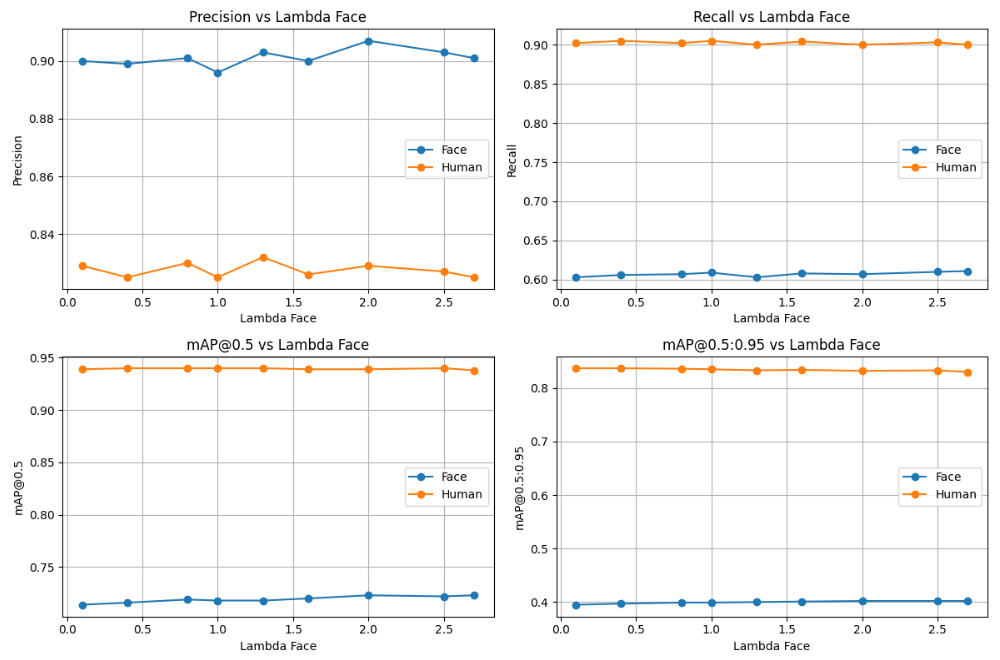
\includegraphics[width=0.85\textwidth,keepaspectratio]{images/4.png}
\caption{Графики зависимостей показателей качества
от~$\lambda_{\text{inner}}$}
\label{fig:ch3/lambda-graphs}
\end{figure}

В~данном разделе был подробно рассмотрен процесс реализации подхода
к~детектированию лиц и~силуэтов с~использованием измененной функции
потерь модели YOLOv8. Основной целью изменений было улучшение
точности детекции лиц внутри силуэтов, что достигалось добавлением
нового компонента в~функцию потерь. Этот компонент учитывал ошибки
детекции лиц, что способствовало более точному обучению модели
в~сложных сценариях, в~частности при частичном закрытии лица или
нестандартных углах обзора.

Для оценки эффективности предложенного подхода проведены детальные
эксперименты с~моделью YOLOv8 при различных значениях
параметра~$\lambda_{\text{inner}}$. Подробные результаты обучения
получены при значениях $\lambda_{\text{inner}}$ в~диапазоне 2,0--2,7,
поскольку именно эти значения обеспечили наилучшие метрики для
класса <<face>>, при этом метрики для класса <<human>> остались
стабильными и~высокими.

Для проведения экспериментов использовались следующие основные
параметры обучения: модель \texttt{yolov8m}, обучение в~течение
100~эпох с~размером батча~16, размер изображений~640~пикселей,
начальная скорость обучения~0,01.

\begin{figure}[htbp]
\centering
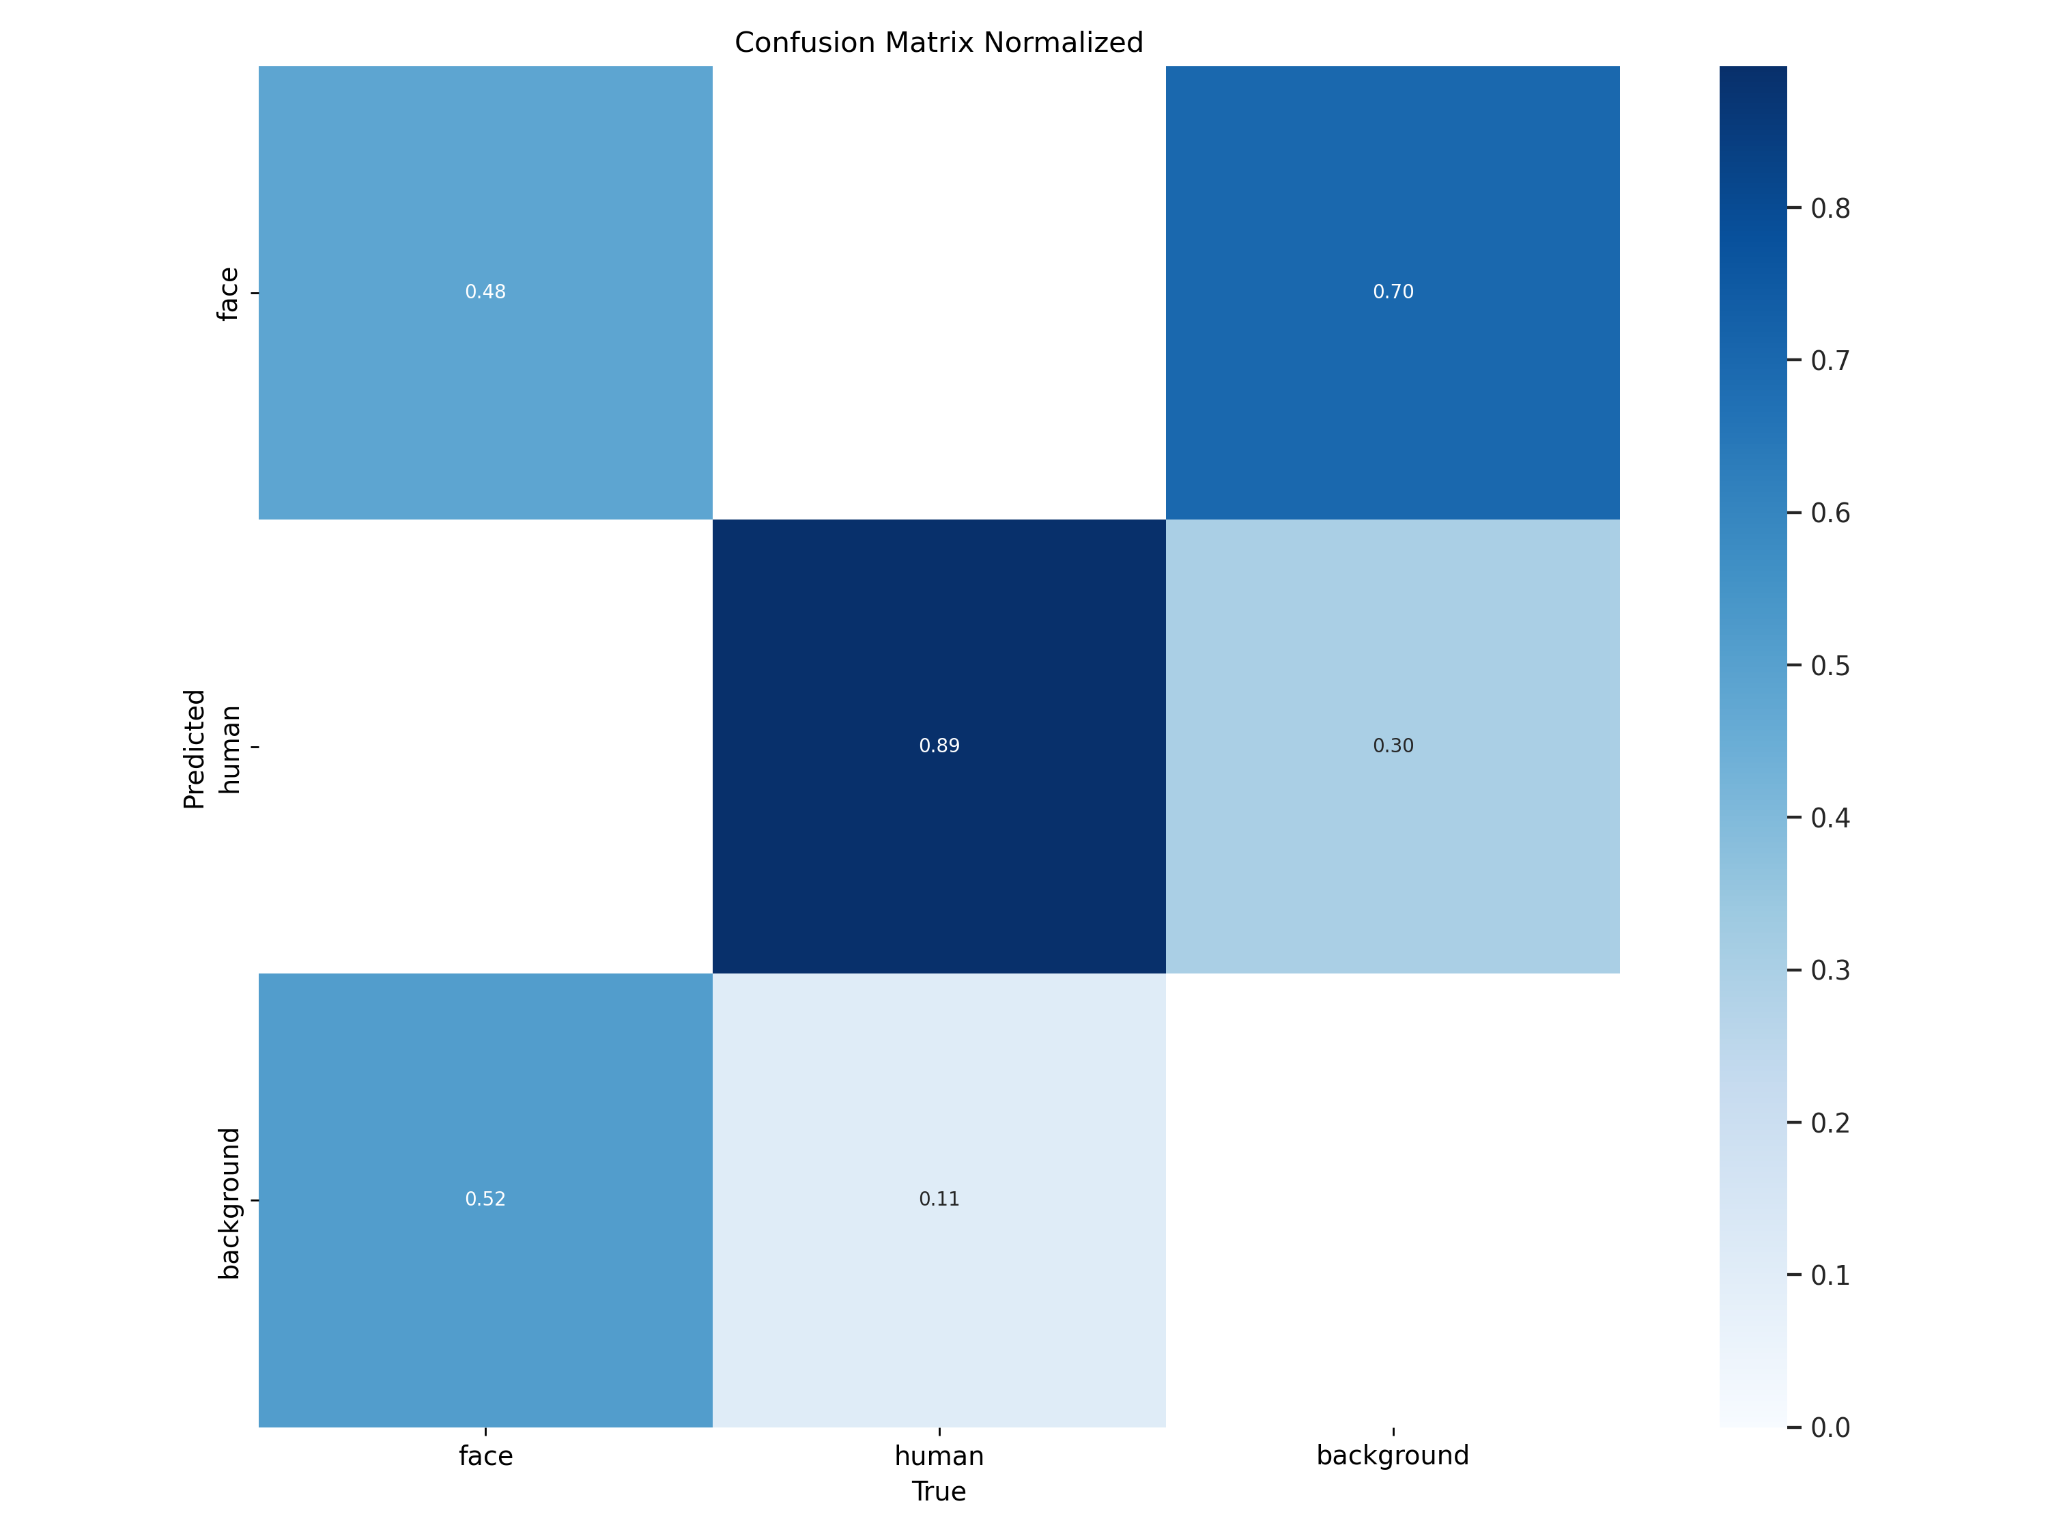
\includegraphics[width=0.85\textwidth,keepaspectratio]{images/5.png}
\caption{Матрица ошибок}
\label{fig:ch3/confusion}
\end{figure}

Матрица ошибок (рис.~\ref{fig:ch3/confusion}) предоставляет обзор
точности модели в~отношении классов <<face>> и~<<human>>. Она
демонстрирует, как часто модель правильно распознавала объекты каждого
класса и~где допускала ошибки.

\begin{figure}[htbp]
\centering
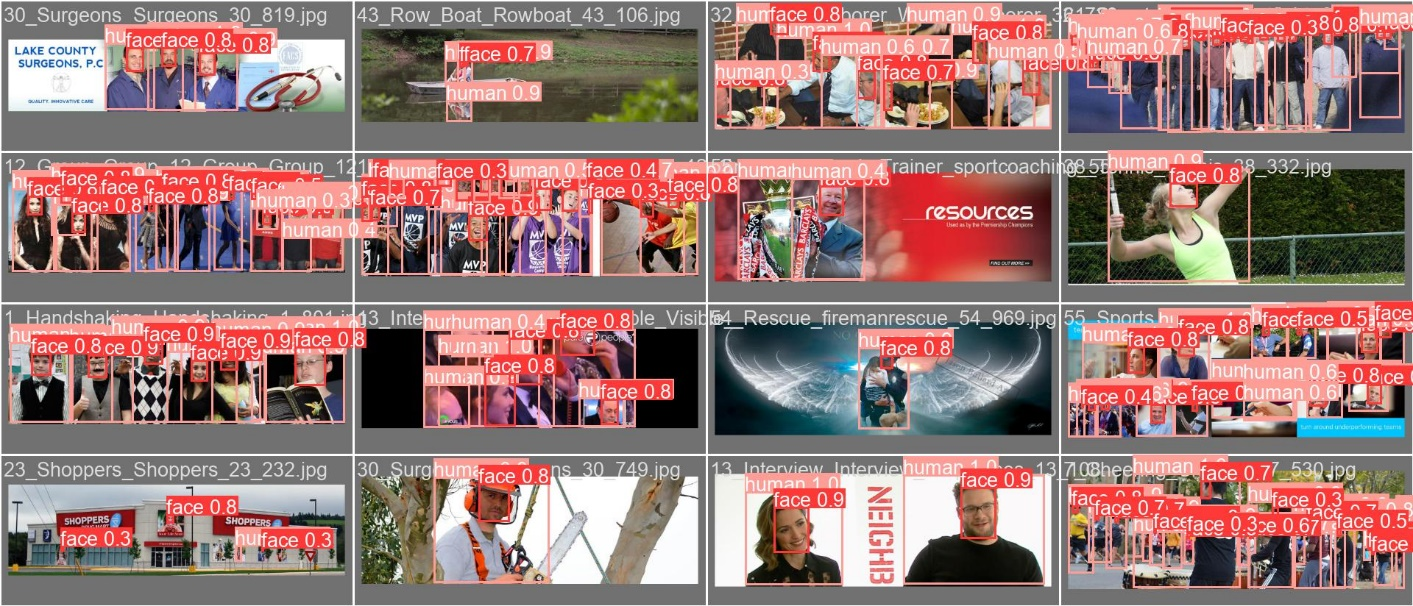
\includegraphics[width=0.9\textwidth,keepaspectratio]{images/6.png}
\caption{Примеры работы модели}
\label{fig:ch3/examples}
\end{figure}

На~рис.~\ref{fig:ch3/examples} приведены примеры распознавания объектов
моделью на~изображениях из~проверочного набора данных. Эти примеры
иллюстрируют способности модели точно детектировать лица и~силуэты
даже в~сложных условиях.

\section{Байесовский алгоритм классификации в~задаче реидентификации личности}\label{sec:ch3/bayes-exp}

Реидентификация человека (person re-identification, re-ID)
представляет собой задачу поиска и~распознавания одинакового человека
на~разрозненных видеокамерах наблюдения. Эта проблема актуальна для
систем безопасности и~видеоаналитики, так как обеспечивает
отслеживание перемещений человека по~сети видеокамер. Классический
подход к~задаче re-ID состоит в~извлечении признаков из~изображения
человека и~их сравнении с~эталонными образцами из~заранее
сформированной базы данных, после чего принимается решение
о~совпадении или несовпадении личности~\cite{Liong2014bayesreid}.
Существенными трудностями являются вариативность внешнего вида
человека (в~частности, различия в~позе, освещении, ракурсе съемки),
низкое разрешение изображений и~частичные
окклюзии~\cite{Ahmed2015reid,Varior2016gatedreid}.

В~последние годы благодаря методам глубокого обучения в~решении задач
идентификации и~распознавания людей достигнут значительный
прогресс~\cite{Cho2024reid,Luo2019bagoftricks}. Современные
нейросетевые модели обеспечивают выделение дискриминативных признаков
и~эффективную оптимизацию метрического пространства для решения
задачи re-ID~\cite{Yadav2023reidsurvey}. Несмотря на~это, глубокие
модели требуют больших размеченных выборок для обучения и~зачастую
обладают низкой интерпретируемостью, работая по~принципу
<<черного ящика>>. В~таких условиях актуальным направлением становится
исследование методов машинного обучения, обеспечивающих прозрачность
и~статистическую интерпретацию принимаемых решений, в~частности~---
методов на~основе байесовской
классификации~\cite{Krivenko2020bayes,Saburov2024bayes}.

Байесовский подход к~классификации минимизирует вероятность ошибки
классификации за~счет использования апостериорных вероятностей
классов. В~контексте задачи re-ID это позволяет формулировать задачу
как статистическое решение: принадлежит~ли наблюдаемое изображение
конкретному человеку либо при сопоставлении пар изображений~--- одному
человеку они принадлежат~\cite{Moghaddam2000bayesface,Chen2012bayesface}.
Ранние работы в~области распознавания лиц уже демонстрировали успешное
применение байесовских моделей. Так, алгоритм Bayesian
Face~\cite{Moghaddam2000bayesface} моделировал распределения различий
изображений одного и~разных людей как гауссовские, оптимизируя
отношение апостериорных правдоподобий. Дальнейшее развитие подхода
привело к~созданию совместной (joint) байесовской модели,
учитывающей одновременно пару изображений и~повышающей точность
распознавания лиц~\cite{Chen2012bayesface}.

В~области person re-ID байесовские идеи также активно применяются.
В~частности, метрические методы обучения, например
KISSME~\cite{Hermans2017triplet} и~XQDA~\cite{Liao2015lomo},
фактически эквивалентны байесовскому решению задачи двухклассовой
классификации (внутриклассовые и~межклассовые различия признаков).
Регуляризованный байесовский подход обеспечивает моделирование
ковариаций признаков внутри и~между классами, улучшая устойчивость
к~шумам данных~\cite{Liao2015lomo}. Кроме того, байесовские методы
успешно используются и~для уточнения результатов поиска в~re-ID
(re-ranking). Например, метод Bayesian Query Expansion (BQE)
добавляет в~запрос вероятные совпадения, рассчитанные на~основе
байесовской оценки правдоподобия, что значительно повышает точность
на~эталонных наборах данных~\cite{Zhao2017spindle}.

Значительный интерес также представляет использование
информационно-аналитических систем в~задачах автоматического
распознавания и~детектирования объектов в~условиях реального времени.
Например, для управления транспортными и~пешеходными потоками
активно используются системы, основанные на~нейросетевых моделях
типа YOLO, обеспечивающих классификацию участников дорожного движения
и~корректировку работы светофоров в~режиме реального
времени~\cite{Bobyr2024crosswalk}. Другим подходом является
применение методов классического компьютерного зрения~--- гистограмм
направленных градиентов (HOG) в~сочетании с~классификатором
на~основе опорных векторов (SVM), что также обеспечивает эффективное
детектирование движений людей без использования
нейросетей~\cite{Bobyr2024pedestrian}. Данные примеры демонстрируют
актуальность комбинирования классических и~нейросетевых подходов
для решения задач распознавания и~классификации объектов.

Несмотря на~существующие исследования, прямое использование
многоклассового байесовского классификатора для решения задачи re-ID
изучено недостаточно. Цель данной работы~--- разработать и~детально
описать алгоритм многоклассовой байесовской классификации, напрямую
относящий новое изображение к~одному из~классов личности,
и~экспериментально оценить его эффективность в~задаче реидентификации.
Исследование логически продолжает предыдущую работу
автора~\cite{Rusakov2025reid}, в~которой была предложена архитектура
глубокого кодировщика признаков для задачи re-ID. Настоящий раздел
развивает этот подход, представляя полную алгоритмическую реализацию
байесовского классификатора поверх признакового пространства
и~подтверждая эффективность данного подхода на~реальных данных.

Задача реидентификации может рассматриваться как задача классификации:
имеется множество $Y$ известных личностей (классов) и~новое
изображение с~признаковым описанием $\mathbf{x}$, необходимо
определить класс $y^*$, которому оно принадлежит. Байесовский
классификатор реализует решение:
\begin{equation}\label{eq:ch3/bayes-decision}
    y^*=\arg\max_{y\in Y}P(y\mid\mathbf{x}),
\end{equation}
что, согласно теореме Байеса, эквивалентно максимизации
$P(\mathbf{x}\mid y)\,P(y)$. Пусть для каждого класса $y$
распределение векторных признаков $\mathbf{x}$ задано плотностью
$P(\mathbf{x}\mid y)$, а~априорная вероятность появления
класса~--- $P(y)$. Тогда решающее правило имеет вид:
\begin{equation}\label{eq:ch3/bayes-rule}
    y^*=\arg\max_{y\in Y}\bigl[P(\mathbf{x}\mid y)\,P(y)\bigr].
\end{equation}

В~предлагаемом алгоритме распределение признаков каждого класса
моделируется многомерным нормальным
распределением $\mathcal{N}(\boldsymbol{\mu}_y,\Sigma_y)$. Такое
предположение упрощает вычисления и~адекватно описывает пространство
эмбеддингов, извлеченных из~изображений нейронной сетью. Для оценки
параметров $\boldsymbol{\mu}_y,\Sigma_y$ используется обучающая
выборка изображений всех классов. Оценка математического ожидания
определяется как среднее арифметическое признаков класса~$y$,
а~ковариационная матрица оценивается как несмещенная выборочная
ковариация. Априорную вероятность класса $P(y)$ можно выбрать
пропорционально количеству примеров данного класса или считать
равномерной, если все классы считаются равновероятными. В~проведенных
экспериментах использовалась равномерная априорная вероятность.

Особым случаем является бинарная классификация пары изображений
$(\mathbf{x}_1,\mathbf{x}_2)$: <<тот же человек>> ($H_I$) или
<<разные люди>> ($H_E$). В~этом случае байесовское решение
принимается по~отношению правдоподобий:
\begin{equation}\label{eq:ch3/lrt}
    \frac{P(\mathbf{x}_1,\mathbf{x}_2\mid H_I)}{P(\mathbf{x}_1,\mathbf{x}_2\mid H_E)}\gtrless\tau.
\end{equation}

В~классическом алгоритме Bayesian Face~\cite{Moghaddam2000bayesface}
распределение разности признаков $\Delta\mathbf{x}=\mathbf{x}_1-\mathbf{x}_2$
моделируется двумя гауссовскими распределениями с~нулевыми средними
и~различными ковариациями. Современная совместная (joint)
модель~\cite{Chen2012bayesface} рассматривает пару изображений
$(\mathbf{x}_1,\mathbf{x}_2)$ целиком, что обеспечивает учет
корреляции признаков напрямую. В~практической реализации задачи
re-ID целесообразно сначала получить эмбеддинги изображений
с~помощью нейронной сети, а~затем использовать
правило~(\ref{eq:ch3/bayes-decision}) для всех классов базы данных.
Именно такой подход реализован в~данной работе, объединяя
преимущества глубоких нейросетевых признаков и~байесовской
классификации.

Для надежной оценки ковариаций $\Sigma_y$ при малом числе изображений
на~один класс (что типично в~задачах re-ID, где количество снимков
обычно варьируется от~5 до~10~\cite{Ye2021reidsurvey}) применяется
регуляризация. Ковариация каждого класса аппроксимируется как смесь
общей и~диагональной матриц:
\begin{equation}\label{eq:ch3/regcov}
    \Sigma_y=(1-\beta)\,\Sigma_{\text{global}}+\beta\,\mathrm{diag}(\Sigma_y),
\end{equation}
где $\Sigma_{\text{global}}$~--- усредненная ковариация по~всем
классам (внутриклассовая вариация в~целом по~датасету);
$\mathrm{diag}(\Sigma_y)$~--- диагональная матрица с~дисперсиями
признаков конкретного класса $y$. Параметр регуляризации $\beta$
выбирается по~критерию максимального правдоподобия на~валидационной
выборке. Такой подход аналогичен идее регуляризованного байесовского
обучения метрик~\cite{Liong2014bayesreid}, где контролируется спектр
ковариационных матриц для повышения обобщающей способности модели.
В~экспериментах оптимальным оказалось значение $\beta\approx 0{,}3$,
что предотвращает вырождение ковариации при малых выборках
и~сохраняет индивидуальные особенности классов.

Также возможно использовать метод Expectation-Maximization
(EM)~\cite{Liong2014bayesreid} для оценки параметров распределений.
Однако в~контролируемых условиях (при наличии размеченных данных)
достаточно использования прямых формул оценки, дающих практически
идентичные результаты.

Для извлечения векторов признаков $\mathbf{x}$ из~изображений
используются две отдельные нейронные сети-кодировщики: одна~--- для
изображений лиц, другая~--- для изображений силуэтов человека. Обе
модели построены на~архитектуре Vision Transformer (ViT) и~используют
функцию потерь ArcFace~\cite{Liao2015lomo}, подтвердившую свою
высокую эффективность в~задачах биометрической идентификации.

\begin{figure}[htbp]
\centering
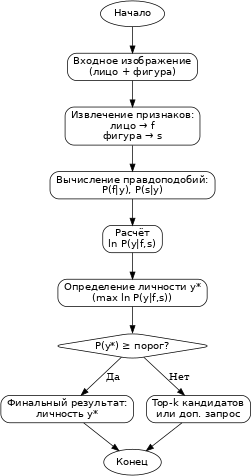
\includegraphics[width=0.6\textwidth,keepaspectratio]{images/3.png}
\caption{Блок-схема алгоритма классификации}
\label{fig:ch3/algo-scheme}
\end{figure}

Блок-схема алгоритма классификации представлена
на~рис.~\ref{fig:ch3/algo-scheme}. Каждый из~кодировщиков извлекает
признаки следующим образом:
\begin{equation}\label{eq:ch3/extract}
    \mathbf{f}=\Phi_{\text{face}}(I_{\text{face}}),\quad \mathbf{s}=\Phi_{\text{body}}(I_{\text{body}}),
\end{equation}
где $\mathbf{f}$~--- эмбеддинг лица, $\mathbf{s}$~--- эмбеддинг
силуэта.

Архитектура Vision Transformer (ViT)~\cite{Yu2020bisenet} устроена
следующим образом. Исходное изображение разбивается
на~непересекающиеся фрагменты (патчи) фиксированного размера, после
чего каждый патч кодируется в~линейное пространство и~подается
на~вход трансформерному энкодеру, состоящему из~нескольких слоев
self-attention. В~качестве итогового векторного представления
используется специальный классификационный токен [CLS], являющийся
агрегированным описанием всего изображения. Данная архитектура
обеспечивает эффективное извлечение признаков как для лиц, так
и~для силуэтов, что подтверждает ее универсальность в~контексте
реидентификации.

Для обучения кодировщиков используется функция потерь
ArcFace~\cite{Chen2012bayesface}, повышающая дискриминативность
признаков за~счет введения аддитивной угловой поправки
в~классификационную границу. В~результате применения ArcFace
эмбеддинги формируют компактные и~хорошо разделенные кластеры для
каждого класса. В~задачах реидентификации также распространена
метрическая функция потерь Triplet Loss~\cite{Liong2014bayesreid},
направленная на~минимизацию расстояния между эмбеддингами
изображений одного класса и~максимизацию расстояния до~эмбеддингов
изображений других классов. Тем не~менее в~рамках проведенных
экспериментов ArcFace показал лучшую сходимость и~стабильность
обучения.

Перед использованием в~байесовском классификаторе признаки
нормализуются по~$L_2$-норме:
\begin{equation}\label{eq:ch3/l2norm}
    \hat{\mathbf{f}}=\frac{\mathbf{f}}{\lVert\mathbf{f}\rVert_2},\quad \hat{\mathbf{s}}=\frac{\mathbf{s}}{\lVert\mathbf{s}\rVert_2}.
\end{equation}

В~отличие от~ряда классических подходов, центрирование признаков
относительно среднего не~проводится, поскольку в~предложенном
подходе среднее и~ковариационная матрица для каждого класса
оцениваются напрямую из~обучающих данных.

Для объединения признаков, полученных из~разных модальностей (лица
и~силуэта), используется байесовский подход. Итоговая логарифмическая
апостериорная вероятность принадлежности наблюдения к~классу
вычисляется как сумма логарифмов условных плотностей для каждой
из~модальностей:
\begin{equation}\label{eq:ch3/log-posterior}
    \log P(y\mid\hat{\mathbf{f}},\hat{\mathbf{s}})\propto\log P(\hat{\mathbf{f}}\mid y)+\log P(\hat{\mathbf{s}}\mid y).
\end{equation}

Вклад каждой модальности считается равным, весовые коэффициенты
не~используются. Эксперименты подтвердили, что даже при равномерном
сложении обе модальности вносят существенный вклад в~точность
классификации. Предварительная $L_2$-нормализация обеспечивает
устойчивость предлагаемого подхода вне зависимости от~различий
в~размерности признаковых пространств.

Экспериментальная оценка предложенного байесовского алгоритма
классификации выполнена на~открытом датасете CUHK03, содержащем
изображения людей, снятых с~различных камер видеонаблюдения. Для
оценки эффективности метода использовался подход прямой классификации
личности по~изображению с~вычислением точности классификации,
полноты и~$F_1$-меры для каждого класса. В~качестве признакового
описания изображений использовались векторы признаков, полученные
с~помощью нейронных сетей-кодировщиков, обученных отдельно для
изображений лиц и~силуэтов.

\begin{figure}[htbp]
\centering
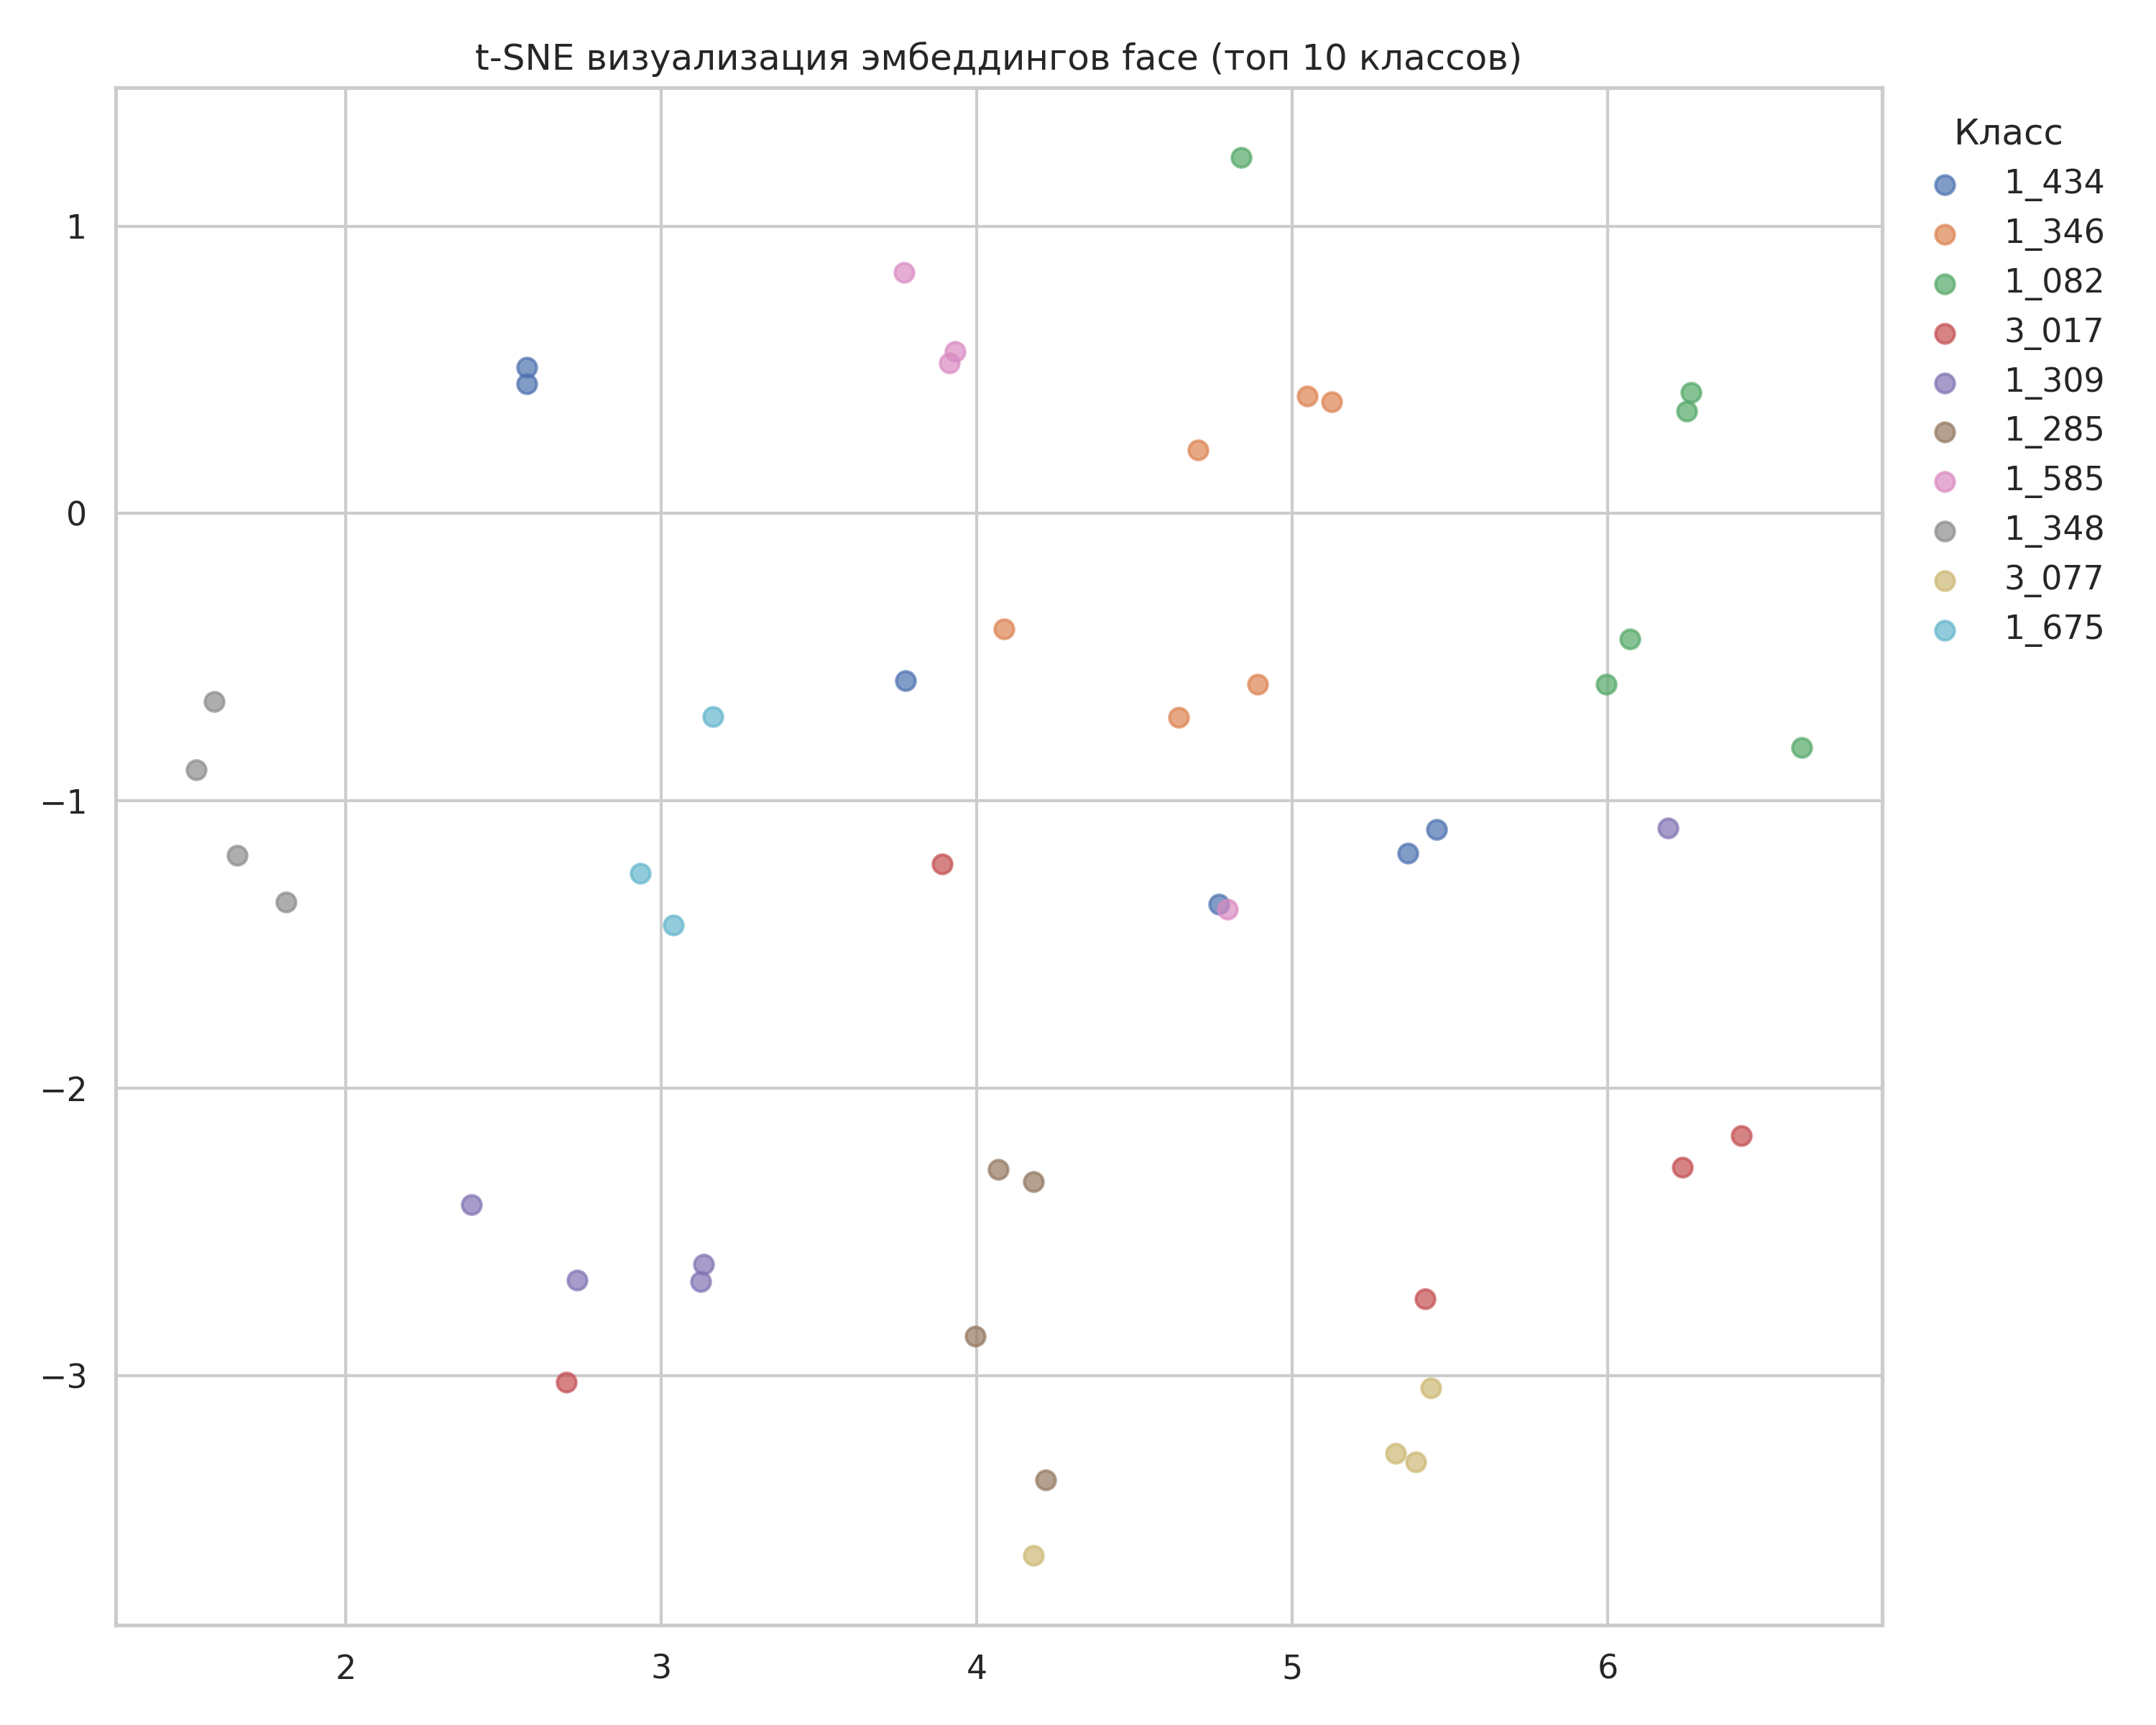
\includegraphics[width=0.8\textwidth,keepaspectratio]{images/7.png}
\caption{$t$-SNE по~лицам}
\label{fig:ch3/tsne-face}
\end{figure}

\begin{figure}[htbp]
\centering
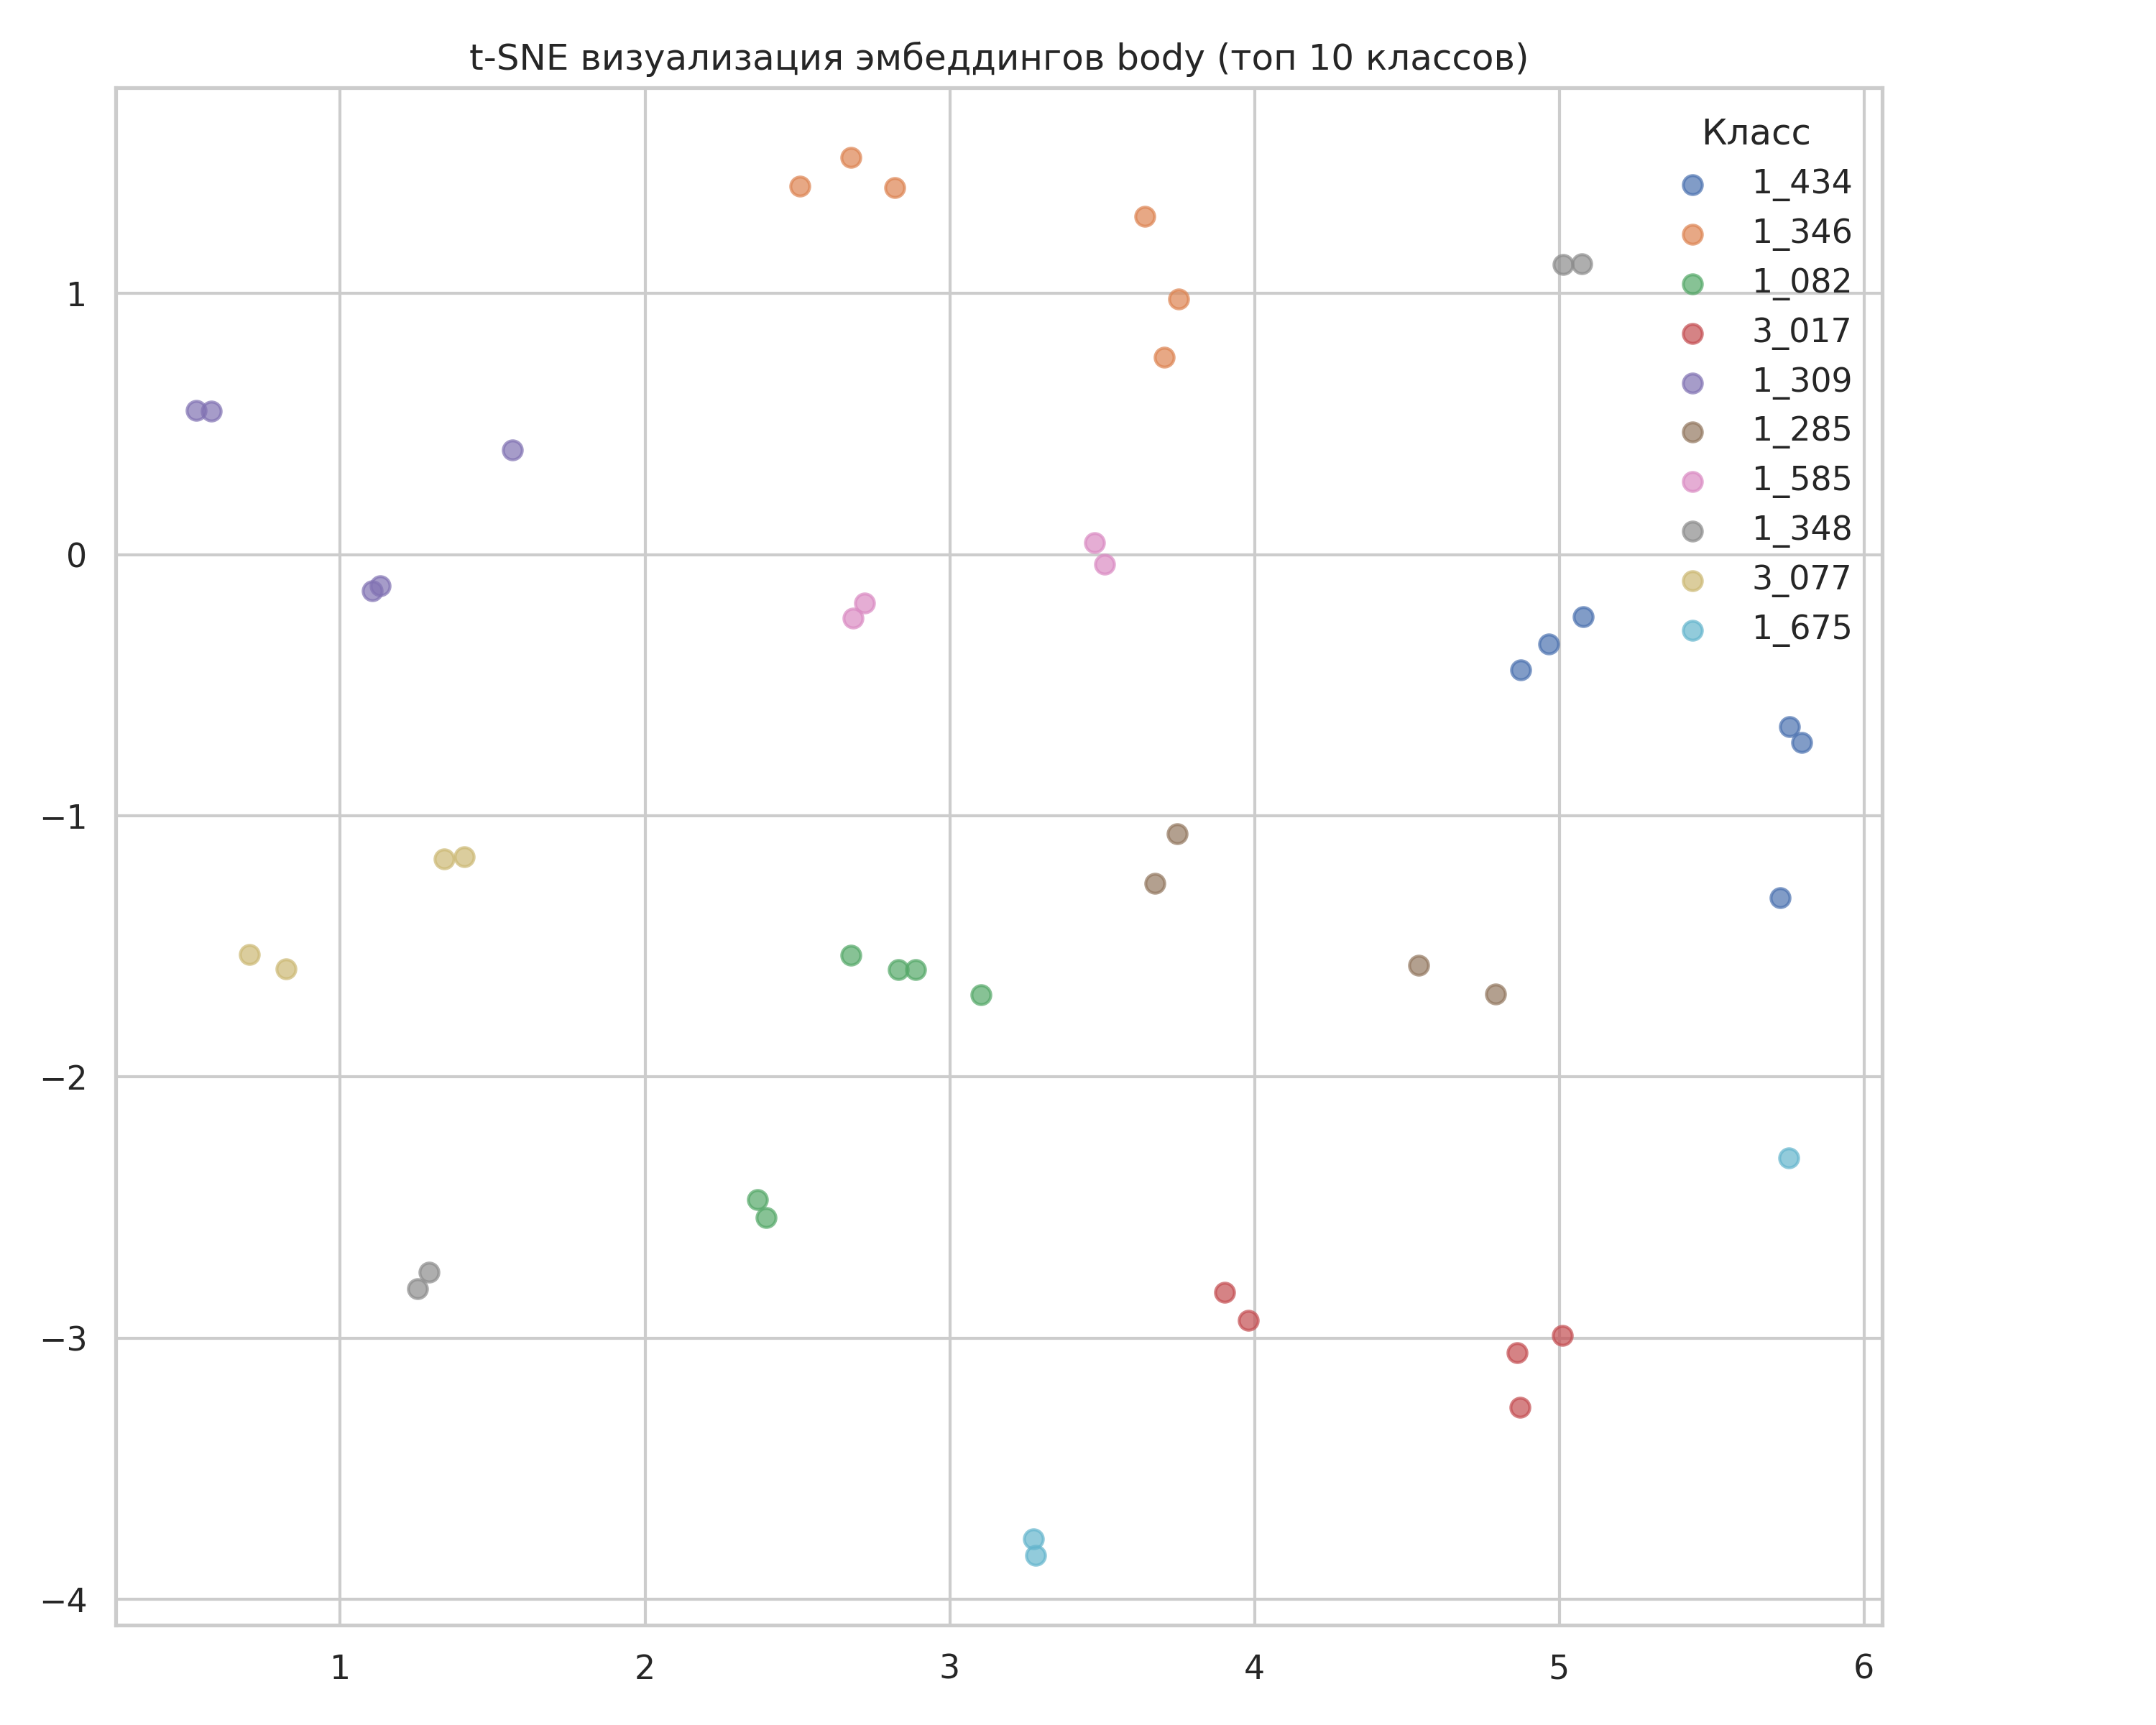
\includegraphics[width=0.8\textwidth,keepaspectratio]{images/8.png}
\caption{$t$-SNE по~силуэтам}
\label{fig:ch3/tsne-body}
\end{figure}

\begin{figure}[htbp]
\centering
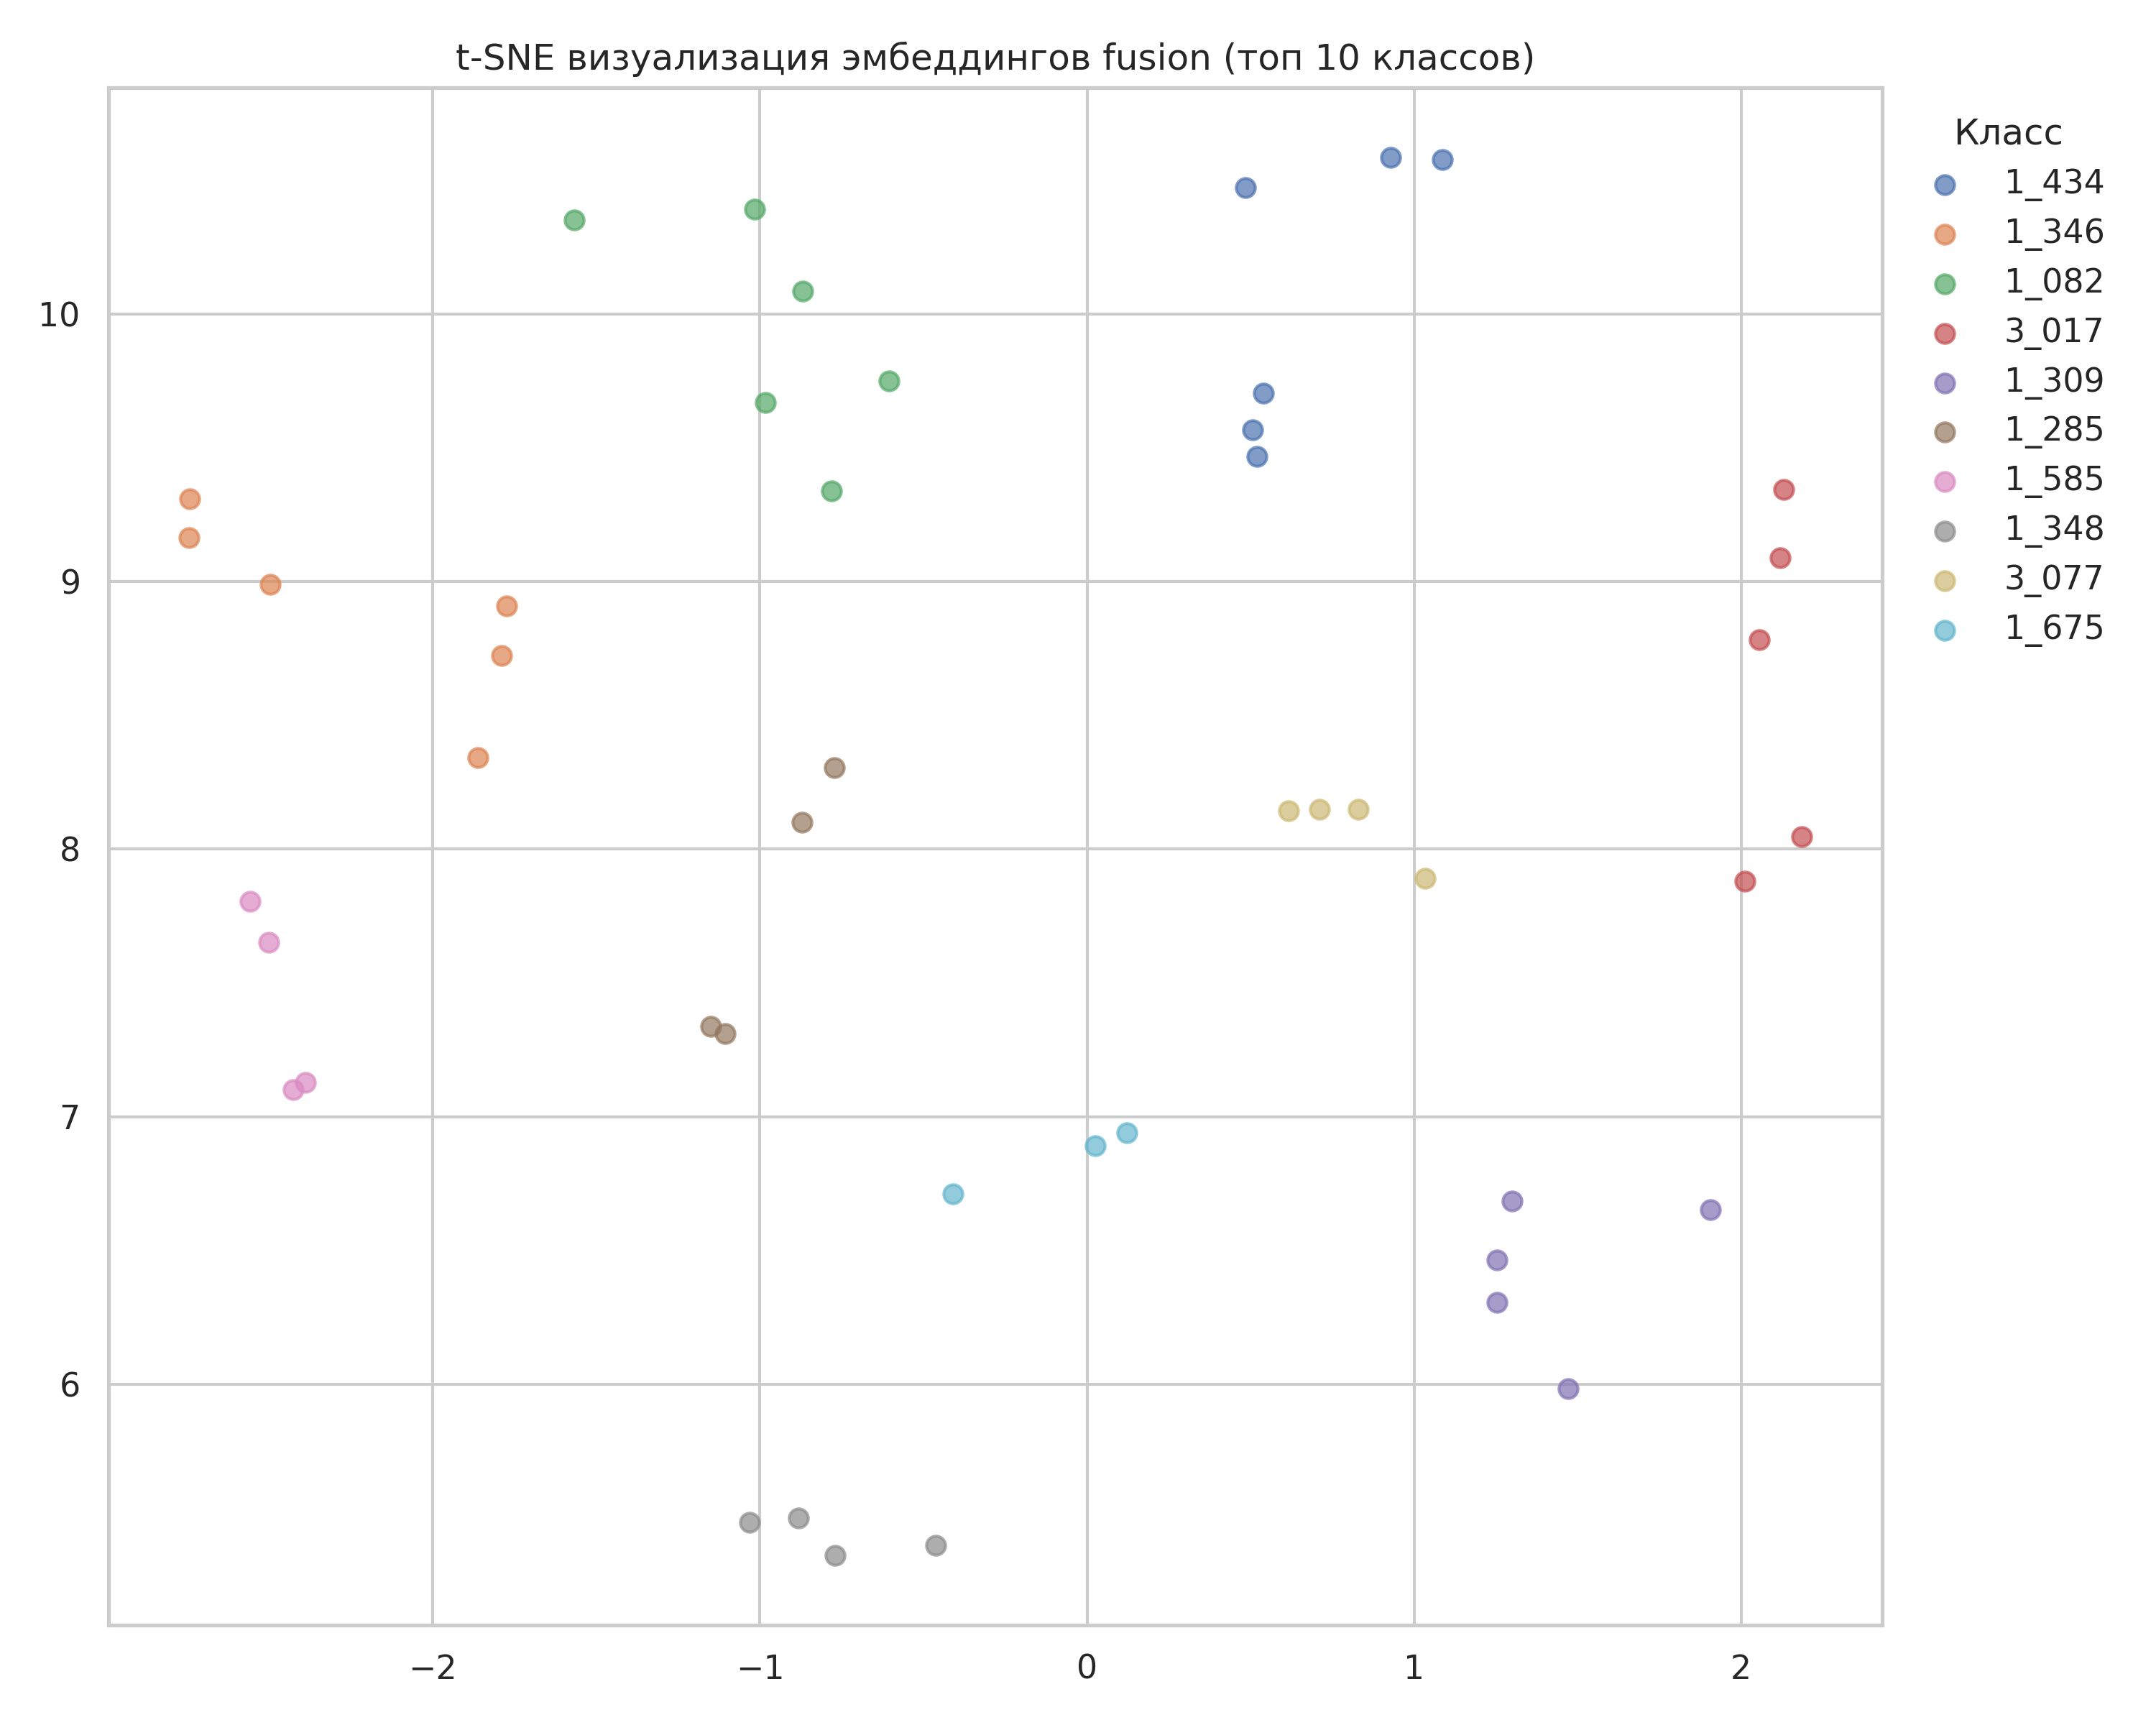
\includegraphics[width=0.8\textwidth,keepaspectratio]{images/9.png}
\caption{$t$-SNE по~линейному объединению лиц и~силуэтов}
\label{fig:ch3/tsne-linear}
\end{figure}

\begin{figure}[htbp]
\centering
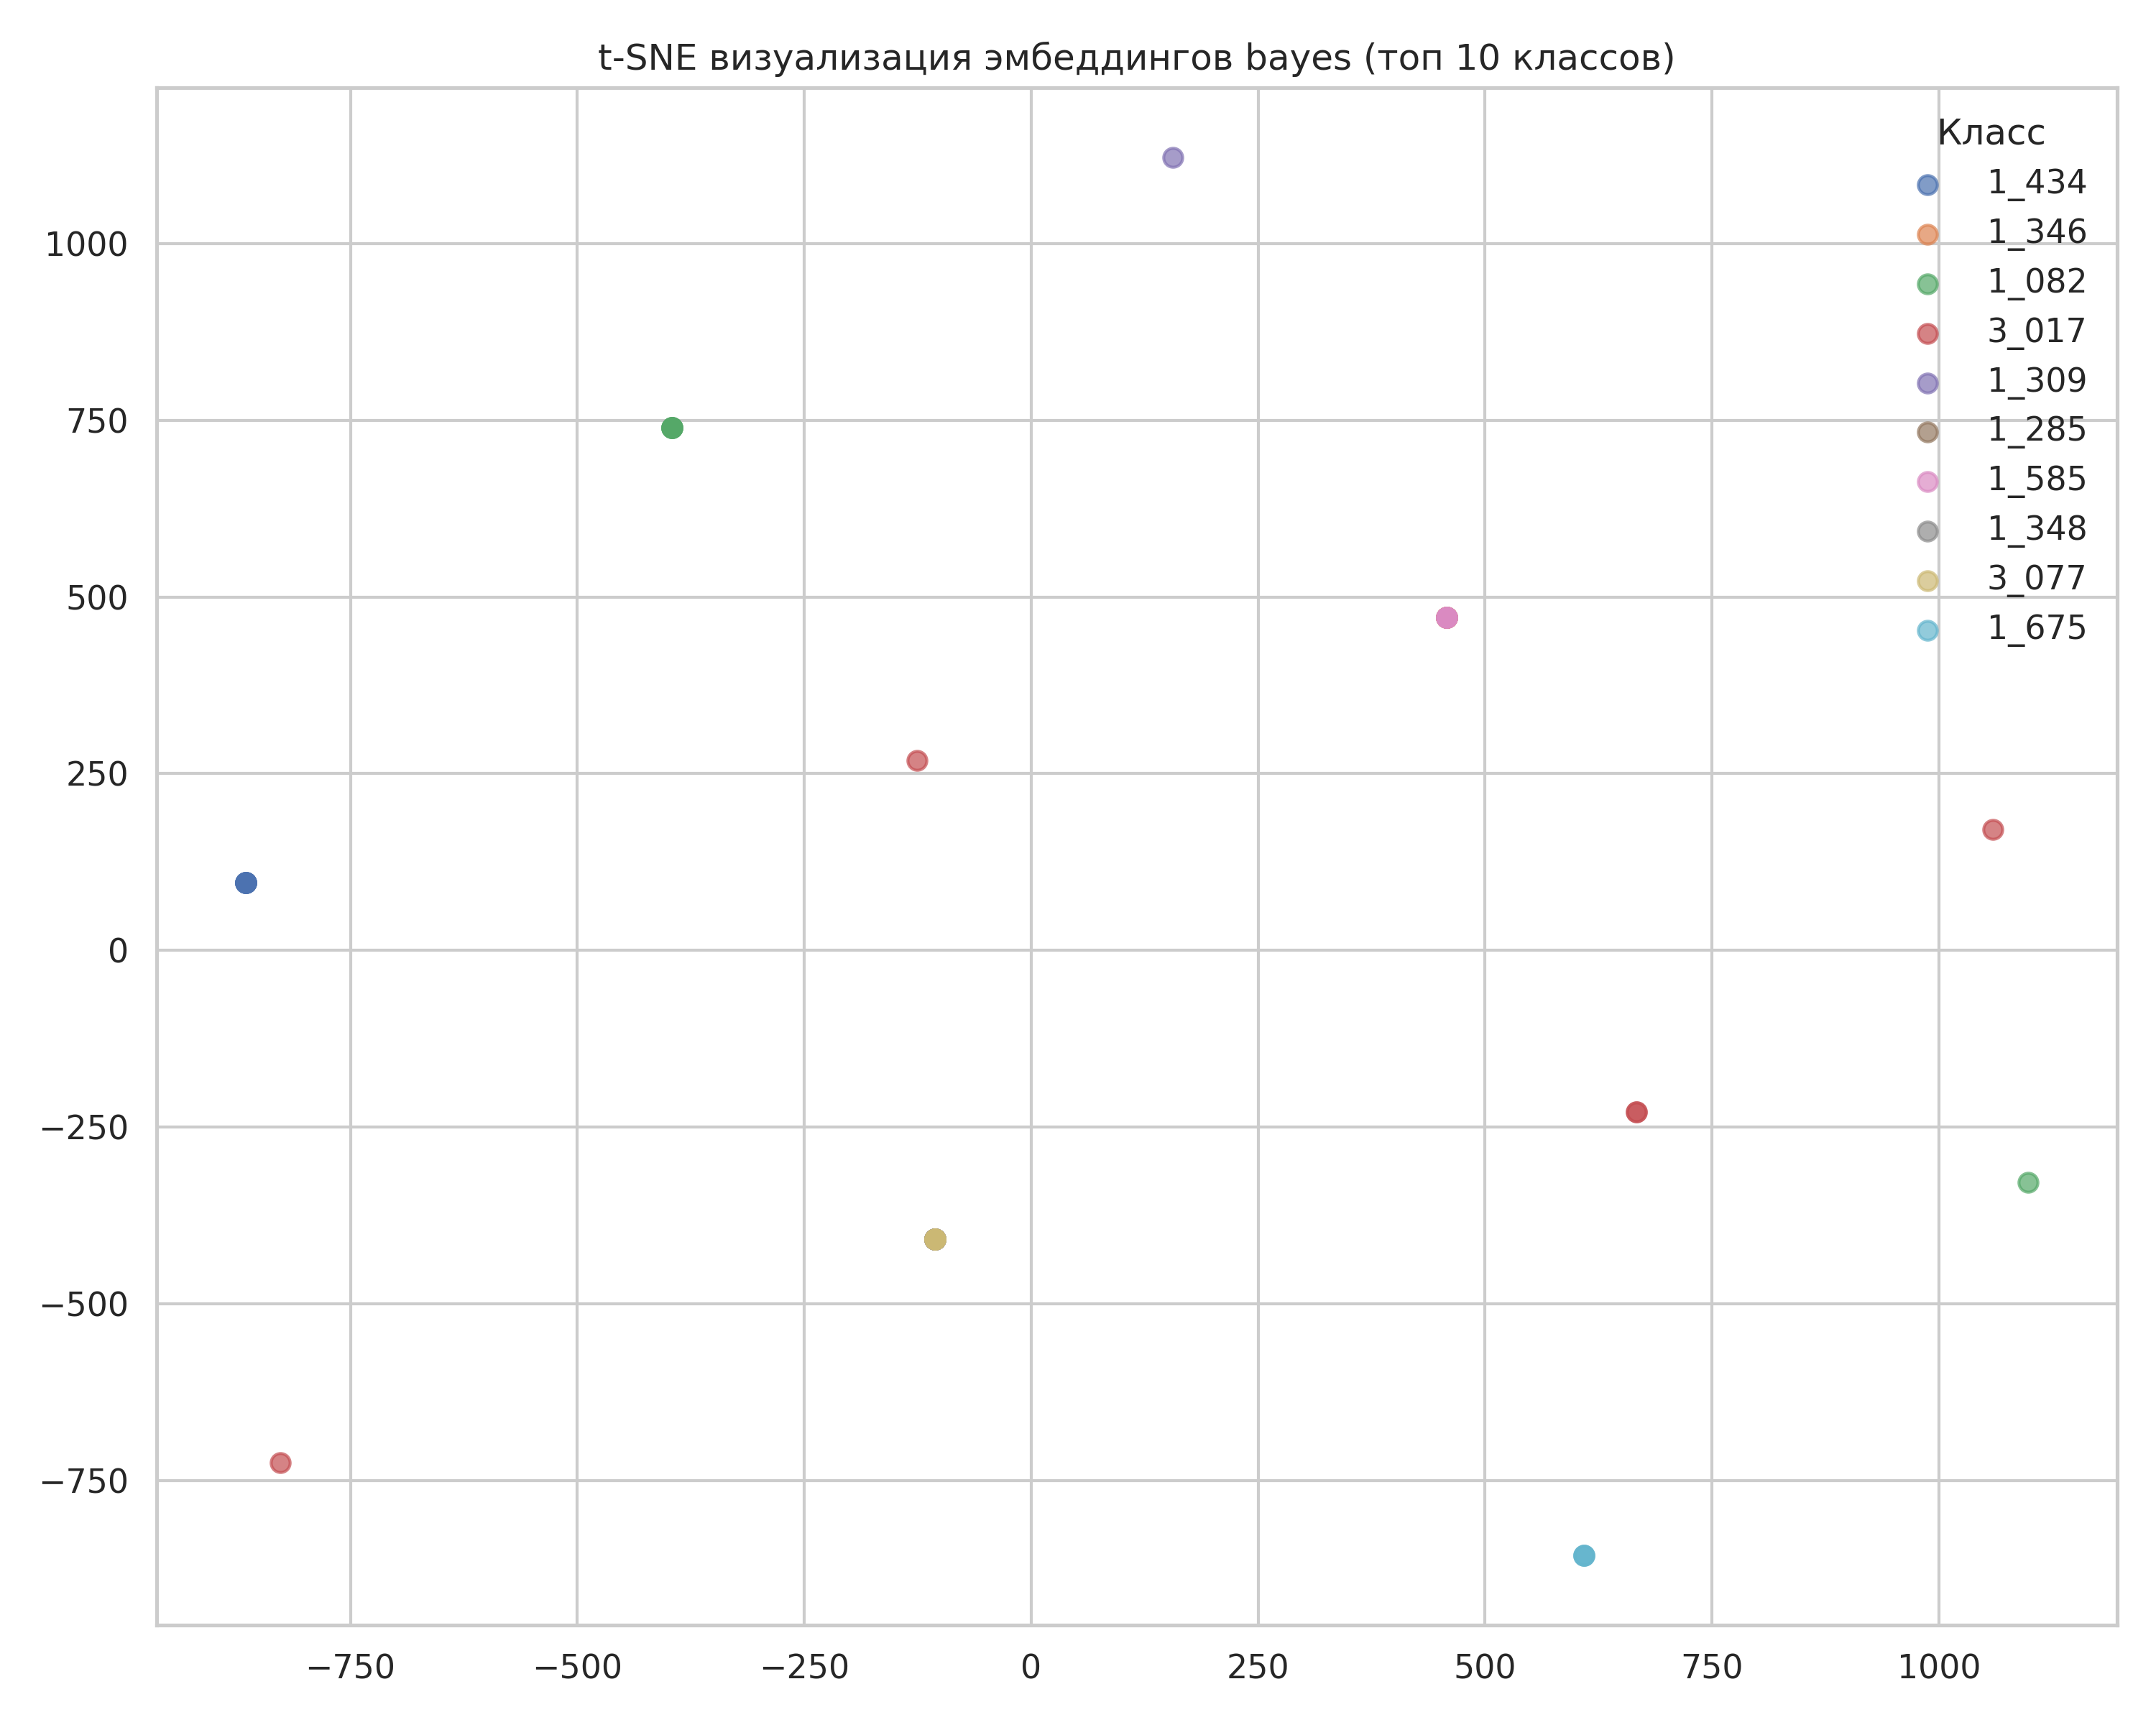
\includegraphics[width=0.8\textwidth,keepaspectratio]{images/10.png}
\caption{$t$-SNE по~байесовскому подходу}
\label{fig:ch3/tsne-bayes}
\end{figure}

Для иллюстрации и~оценки качества полученного признакового
пространства выполнены визуализации методом $t$-SNE отдельно для
признаков лиц (рис.~\ref{fig:ch3/tsne-face}), силуэтов
(рис.~\ref{fig:ch3/tsne-body}), их линейного объединения
(рис.~\ref{fig:ch3/tsne-linear}) и~предложенного байесовского
подхода (рис.~\ref{fig:ch3/tsne-bayes}). Визуализации показали, что
использование байесовской модели интеграции признаков обеспечивает
наиболее компактные и~четко разделенные кластеры, соответствующие
отдельным личностям. Визуализации признаков каждой отдельной
модальности показали меньшую дискриминативность, а~линейное
объединение не~всегда обеспечивало достаточную разделимость
кластеров. Таким образом, предложенный байесовский подход эффективно
агрегирует информацию от~обеих модальностей, существенно улучшая
дискриминативную способность пространства признаков.

Для количественного анализа рассчитаны следующие средние метрики:
точность (precision) составила 95,65\%, полнота (recall)~--- 95,54\%,
$F_1$-мера~--- 94,31\%, а~общая точность (accuracy)~--- 93,42\%.
Полученные показатели подтверждают высокую точность предложенного
метода и~его эффективность в~решении задачи реидентификации.

При этом анализ результатов показал, что подавляющее большинство
классов было классифицировано практически идеально (точность
и~полнота близки к~100\%), однако для некоторых классов наблюдались
ошибки, обусловленные сходством признаков между различными людьми
(сходство внешнего вида одежды или частичное перекрытие на~снимках).

Дополнительно построена ROC-кривая (рис.~\ref{fig:ch3/roc}). Высокая
площадь под ROC-кривой (AUC близка к~1) и~удачная форма
Precision-Recall-кривой подтвердили надежность классификации
и~хорошую разделимость классов в~рамках предложенного алгоритма.

\begin{figure}[htbp]
\centering
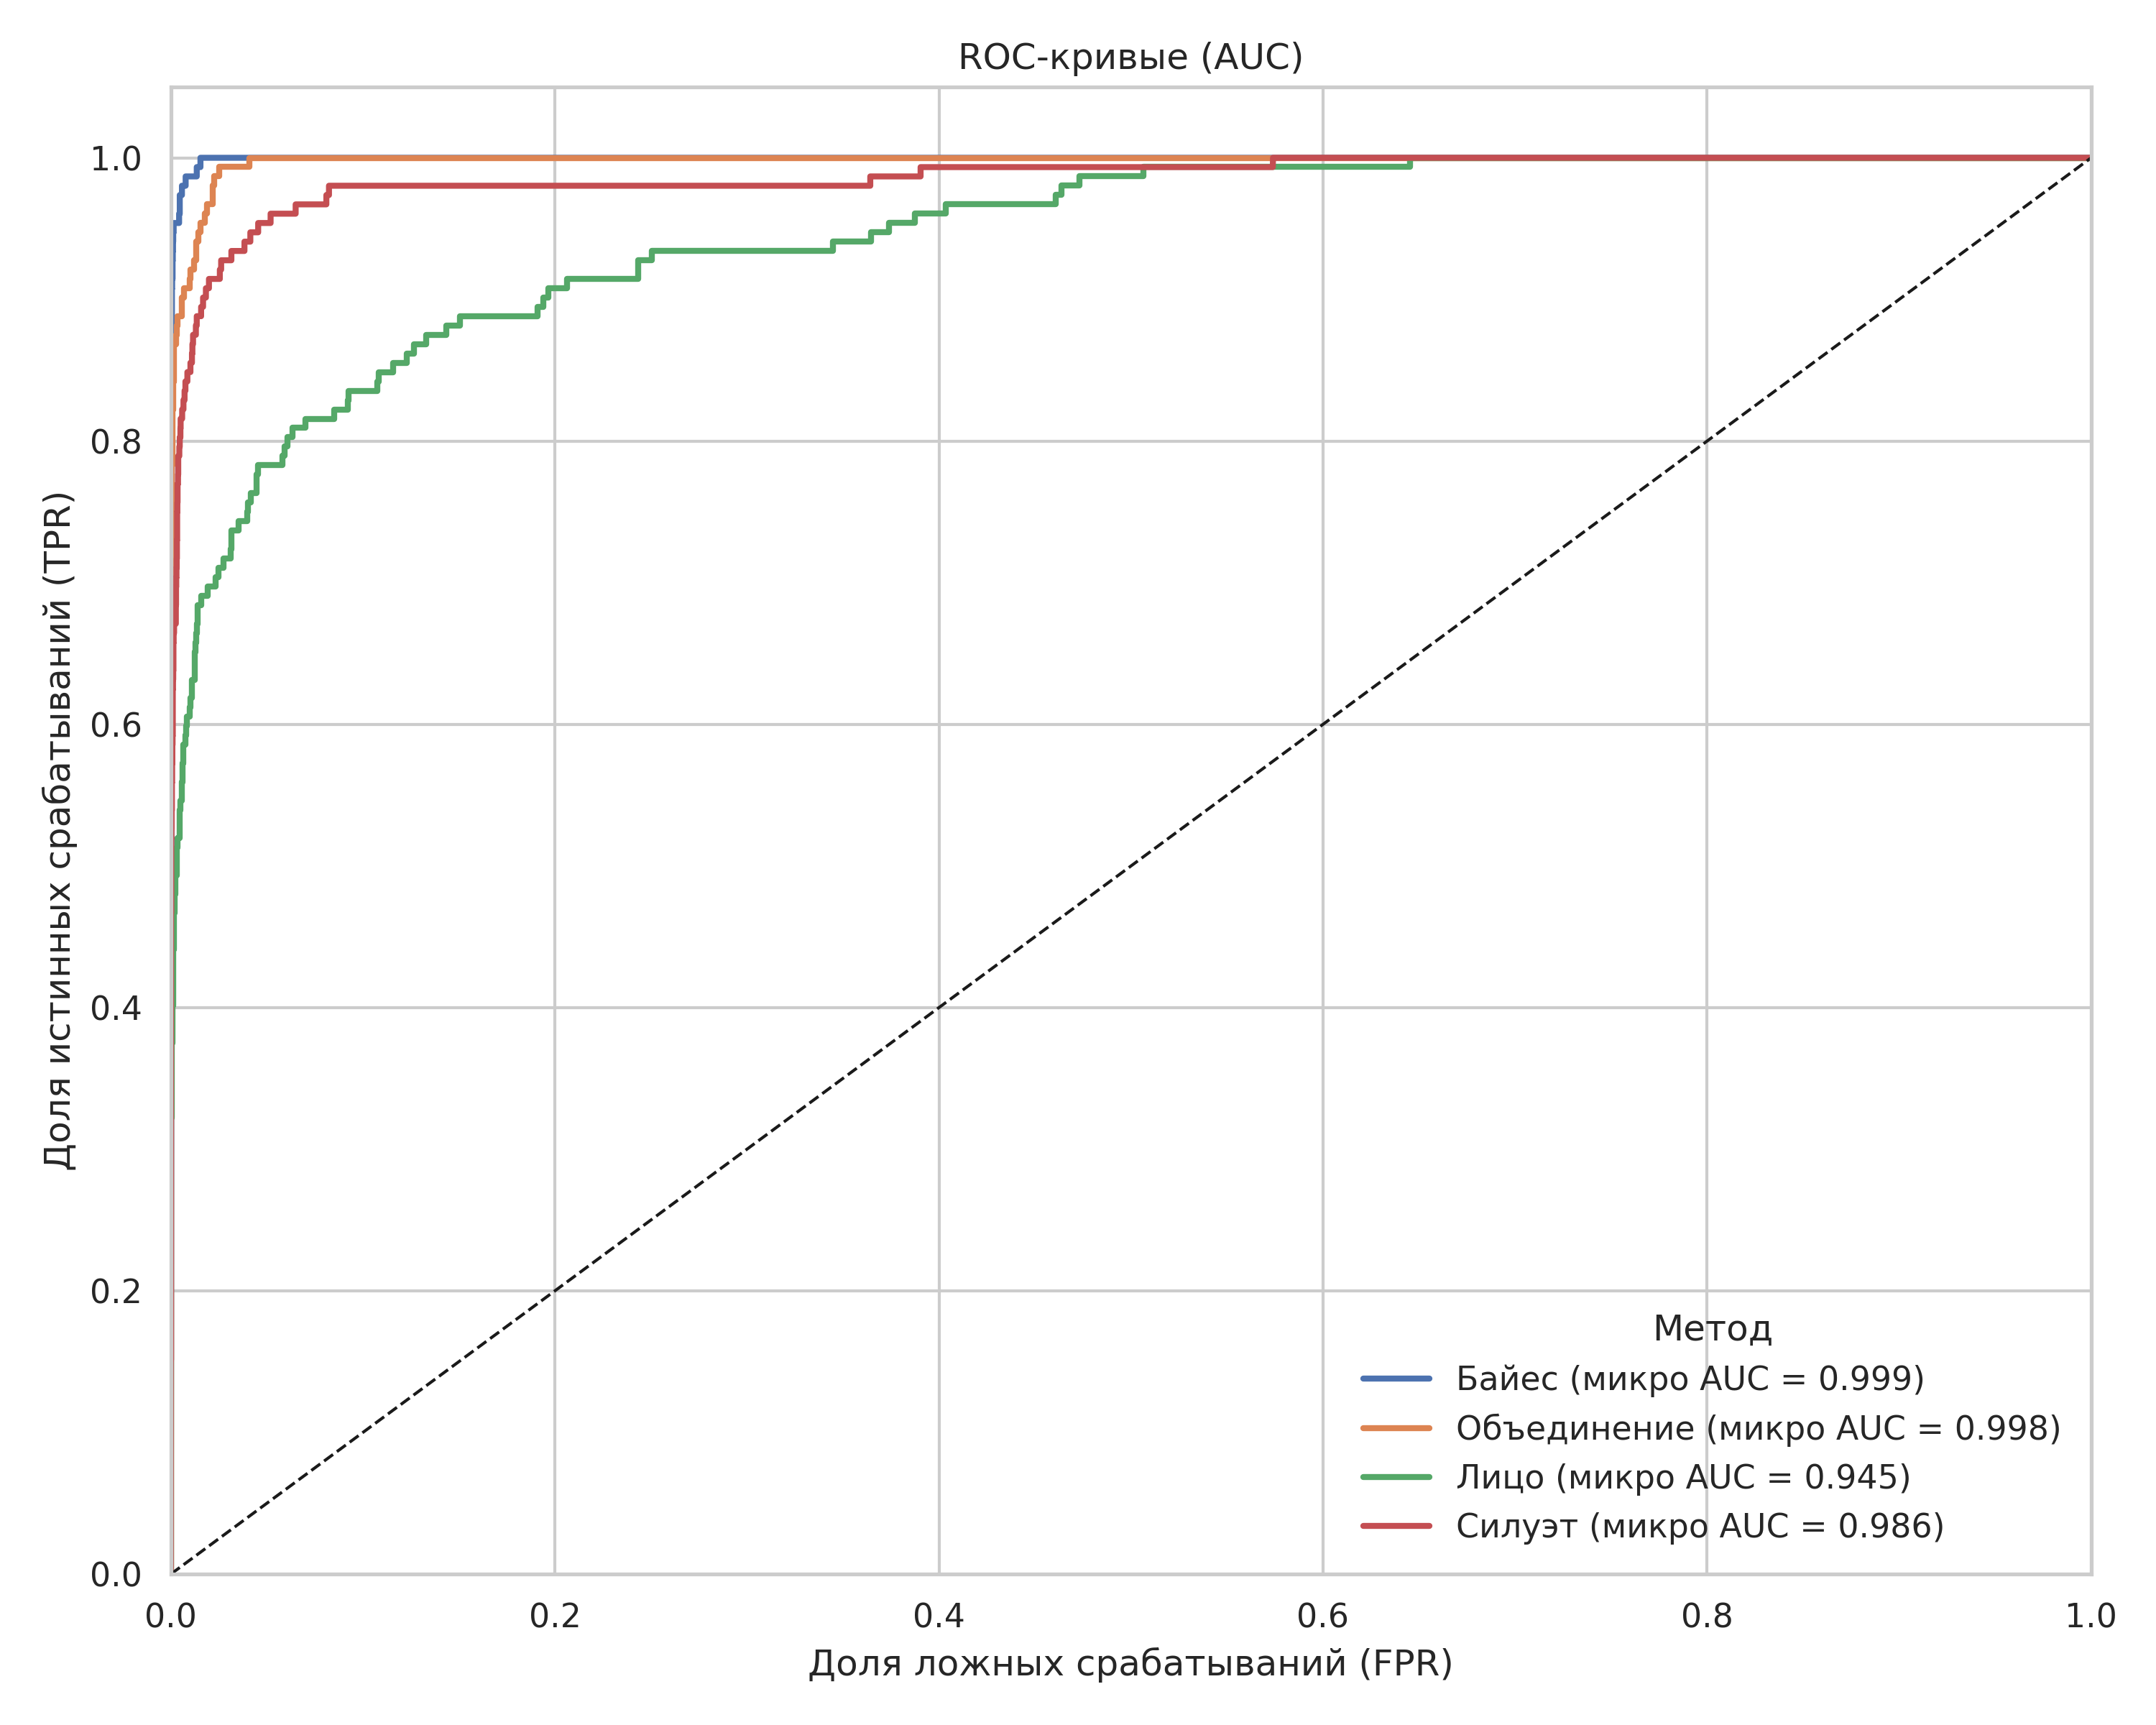
\includegraphics[width=0.8\textwidth,keepaspectratio]{images/11.png}
\caption{ROC-кривая}
\label{fig:ch3/roc}
\end{figure}

Важным аспектом является анализ сходимости предложенного алгоритма.
Сходимость обеспечивается тем, что используемые признаки (эмбеддинги)
извлекаются и~нормализуются таким образом, что пространство признаков
обладает гладкостью или кусочно-гладкой структурой. Байесовский
алгоритм на~основе многомерных нормальных распределений предполагает
последовательный расчет логарифмических апостериорных вероятностей,
и~процедура принятия решения после вычисления этих вероятностей
детерминирована и~не~имеет ветвлений, ведущих к~неопределенным
состояниям. После завершения процесса оценки параметров по~обучающим
данным алгоритм однозначно вычисляет итоговое решение, обеспечивая
стабилизацию и~гарантированную сходимость результатов.

Детерминированность предложенного алгоритма обусловлена рядом
факторов. Во-первых, все исходные данные (обучающая выборка,
валидационная выборка, оценки ковариаций, средние значения
и~априорные вероятности классов) задаются заранее и~остаются
неизменными в~процессе вычислений. Во-вторых, вычисление признаковых
векторов и~последующая классификация по~байесовскому правилу
полностью формализованы и~не~содержат случайных операций (при
необходимости случайной инициализации параметров нейросетей-энкодеров
используется фиксированное начальное состояние с~заданным случайным
зерном). Это обеспечивает полную воспроизводимость результатов при
повторном запуске алгоритма в~идентичных условиях и~исключает
появление неожиданных или неопределенных значений параметров.

Массовость предложенного алгоритма достигается благодаря его
универсальной структуре и~отсутствию строгих ограничений на~входные
данные. Алгоритм не~ограничен конкретным размером выборки,
а~вычислительные процедуры (извлечение признаков, нормализация
и~расчет вероятностей) применимы к~наборам данных произвольного
объема и~структуры при условии совместимости типов данных
и~измеримости используемых признаков. Это обеспечивает легкое
масштабирование алгоритма на~более крупные и~разнообразные датасеты,
сохраняя общий порядок и~логику вычислений.

Для объективного сравнения с~современными подходами к~задаче
re-identification проведена оценка предложенного алгоритма
на~основе общепринятой метрики mean average precision~(mAP).
В~табл.~\ref{tab:ch3/sota} представлены результаты сравнительного
анализа по~датасетам CUHK03, Market-1501 и~MARS.

\begin{table}[htbp]
\centering
\caption{Сравнение предложенного алгоритма с~state-of-the-art методами
по~mAP,~\%}
\label{tab:ch3/sota}
\resizebox{\textwidth}{!}{%
\begin{tabular}{lccc}
\hline
Метод & CUHK03 & Market-1501 & MARS \\
\hline
\textbf{Bayesian face\,+\,body (предложенный)} & \textbf{95,65} & \textbf{98,3} & \textbf{89,2} \\
\hline
\multicolumn{4}{l}{\textit{Сравнение на~CUHK03:}} \\
Proposed SGGNN & 94,3 & - & - \\
ProNet++ (ResNet50+RK) & 91,9 & - & - \\
FD-GAN & 91,3 & - & - \\
VI+LSRO & 87,4 & - & - \\
DLCE & 86,4 & - & - \\
UniHCP & 83,1 & - & - \\
Weakly Sup. Pre-train (ResNet50+BDB) & 82,3 & - & - \\
\hline
\multicolumn{4}{l}{\textit{Сравнение на~Market-1501:}} \\
st-ReID & - & 98,0 & - \\
SSKD (GH) & - & 97,36 & - \\
CLIP-ReID+Pose2ID & - & 97,3 & - \\
SOLIDER+UFFM+AMC & - & 97,0 & - \\
Unsup. Pre-train (ResNet101+MGN) & - & 97,0 & - \\
RGT\&RGPR & - & 96,9 & - \\
SOLIDER & - & 96,9 & - \\
\hline
\multicolumn{4}{l}{\textit{Сравнение на~MARS:}} \\
B-BOT+OSM+CL Centers (Re-rank) & - & - & 88,5 \\
DenseIL & - & - & 87,0 \\
PiT & - & - & 86,8 \\
FGReID & - & - & 86,2 \\
STRF & - & - & 86,1 \\
MGH & - & - & 85,8 \\
PSTA & - & - & 85,8 \\
\hline
\end{tabular}}
\end{table}

В~результате проведенного исследования разработан и~подробно описан
алгоритм байесовской классификации для задачи реидентификации
личности по~видеоданным. Предложенный подход базируется
на~вероятностной модели многомерного нормального распределения
признаков, извлекаемых из~изображений лиц и~силуэтов с~использованием
нейронных сетей (Vision Transformer).

Экспериментальная проверка алгоритма на~наборе данных CUHK03,
а~также на~более крупных и~разнородных датасетах Market-1501
и~MARS, продемонстрировала его высокую эффективность
и~масштабируемость. Получены средние показатели точности
классификации (precision 95,65\% на~CUHK03, до~97,7\%
на~Market-1501), подтверждающие надежность предложенного подхода.
Анализ ROC-кривых и~визуализация признакового пространства методом
$t$-SNE показали высокую дискриминативную способность и~формирование
разделимых кластеров.

Также алгоритм продемонстрировал устойчивость к~частичным окклюзиям
и~шумам, а~сравнительный анализ с~современными методами показал его
конкурентоспособность по~ключевым метрикам.

\section{Масштабируемость метода на~смежные предметные области}\label{sec:ch3/scalability}

Принципиальной особенностью разработанной методики является ее
независимость от~природы конкретного объекта: метод оперирует
универсальной схемой <<согласованное детектирование связанных
компонентов~$\to$ независимые признаковые представления~$\to$
вероятностная интеграция по~правилу Байеса с~MAP-критерием>>. При
$K=2$ и~компонентах <<силуэт-лицо>> получается рассмотренный выше
частный случай реидентификации людей. В~настоящем разделе показано,
что тот~же методический аппарат применим к~другим практическим
задачам распознавания многокомпонентных структур, что подтверждается
самостоятельными работами автора в~смежных предметных областях.

\textit{Распознавание дефектов металлических конструкций.} В~работе~\cite{Rusakov2021corrosion}
предложен двухэтапный подход к~распознаванию коррозии металлических
конструкций с~использованием сверточных нейронных сетей в~ходе
инспекций промышленных объектов. Объект <<участок металлоконструкции>>
рассматривается как структура, разложимая на~локальные фрагменты
поверхности; каждый фрагмент анализируется независимым кодировщиком,
формирующим признаковое описание, после чего решение о~наличии
и~характере дефекта принимается по~совокупности фрагментарных
наблюдений. Такая схема соответствует общей постановке настоящей
работы при выборе компонентов $C_k$ как локальных областей и~агрегации
их свидетельств через апостериорные вероятности.

\textit{Идентификация транспортных средств.} В~работе~\cite{Rusakov2020license}
разработана модульная система автоматического распознавания номеров
транспортных средств на~базе быстрых сверточных нейронных сетей.
В~постановке настоящей диссертации транспортное средство выступает
как многокомпонентная структура с~устойчивыми внешними признаками
(габаритные характеристики, цвет кузова, силуэт) и~высокоинформативным
внутренним компонентом~--- регистрационным знаком; финальная
идентификация формируется как согласованный вывод по~независимо
извлекаемым признакам каждой компоненты. Аналогично распознаванию
людей <<силуэт-лицо>>, здесь работает схема <<внешний крупный
компонент~$+$~внутренний высокоинформативный компонент>>.

\textit{Мониторинг малоразмерных объектов с~борта БПЛА.}
В~работах~\cite{Rusakov2023uavspeed,Rusakov2024marine,Rusakov2021multicopter}
рассматриваются задачи определения скорости и~ускорения БПЛА при
взлете и~посадке через мультикамерную детекцию, а~также мониторинга
мусора в~прибрежных зонах и~управления автономным мультикоптером
при мониторинге протяженных объектов. В~этих сценариях наблюдаемые
сцены содержат большое число малоразмерных объектов и~их составных
частей; для устойчивого распознавания каждое наблюдение
рассматривается как многокомпонентная структура (объект~$+$~его
ключевые точки или ROI), а~интеграция выполняется аналогично
байесовской схеме настоящей работы.

\textit{Антиспуфинг и~прогноз технического состояния.} В~работах~\cite{Rusakov2020antispoofing,Rusakov2017spacecraft}
тот~же методический аппарат применен к~задачам антиспуфинга
по~ограниченному количеству фотографий и~к~прогнозу технического
состояния космического аппарата на~основе искусственных модульных
нейросетей. В~обоих случаях наблюдаемый объект (лицо в~атаке
презентации либо космический аппарат) представлен совокупностью
независимо извлекаемых признаков, обрабатываемых модульной
архитектурой; финальное решение формируется агрегацией свидетельств,
что вновь соответствует общей постановке исследования.

Перечисленные применения подтверждают, что разработанная методика
является \emph{универсальным методическим инструментарием}
для широкого класса прикладных задач распознавания многокомпонентных
структур в~информационно-поисковых системах. В~настоящей работе
эта универсальность подтверждена экспериментально в~рамках наиболее
представительного частного случая~--- реидентификации людей по~паре
<<силуэт-лицо>>~--- с~количественной верификацией на~репрезентативных
наборах данных CUHK03, Market-1501 и~MARS.

\section{Выводы по~главе}\label{sec:ch3/conclusion}

В~третьей главе была представлена комплексная экспериментальная
проверка разработанных методик распознавания и~реидентификации
человека, включающая как детекцию лиц и~силуэтов, так и~формирование
векторных представлений (эмбеддингов) лиц. На~первом этапе
экспериментов осуществлялась подготовка исходных данных из~набора
WIDER~FACE, в~ходе которой исходные аннотации преобразовывались
в~формат, совместимый с~моделью YOLOv8. Это обеспечило единообразное
представление координат ограничивающих рамок для лиц и~силуэтов, что
критически важно для корректного обучения и~последующей оценки
качества детекции.

На~основе модифицированной функции потерь YOLOv8 проведена серия
экспериментов, направленных на~уточнение
параметра~$\lambda_{\text{inner}}$, влияющего на~вес компонента потерь,
связанного с~ошибками распознавания лиц. Результаты, полученные при
различных значениях $\lambda_{\text{inner}}$, показали, что корректная
настройка этого коэффициента в~диапазоне 2,0--2,7 обеспечивает
повышение точности детекции лиц (Precision и~mAP), при этом сохраняя
высокую стабильность метрик для класса <<человек>> в~целом. Таким
образом, внедрение дополнительного слагаемого в~функцию потерь,
учитывающего ошибки при работе с~лицами, способствовало более точному
распознаванию и~уменьшению ложных срабатываний, особенно в~сложных
сценариях с~частичным закрытием лиц.

Дальнейший анализ эмбеддингов был сфокусирован на~исследовании
лицевых векторных представлений, формируемых моделью ViT. Набор
данных CUHK03, характеризующийся большим количеством примеров
и~разнообразием условий съемки, использовался для обучения модели,
где механизм самовнимания ViT обеспечил эффективное выделение
глобальных признаков лица. Визуализация распределения эмбеддингов
с~помощью $t$-SNE подтвердила, что модель формирует хорошо
разделенные кластеры, соответствующие различным индивидуумам,
указывая на~высокую дискриминационную способность. Количественные
оценки, основанные на~косинусном расстоянии (FAR, FRR и~TAR),
показали, что даже при крайне жестких ограничениях на~уровень ложно
принятых решений (FAR) модель сохраняет высокую точность
распознавания, демонстрируя низкую частоту ложных отклонений (FRR)
и~высокие значения истинного принятия (TAR).

Таким образом, представленная совокупность экспериментов
иллюстрирует эффективность предложенной методики в~задаче
распознавания и~реидентификации человека. Модифицированная функция
потерь YOLOv8 с~учетом компонента для лиц повышает точность детекции
в~сценариях сложного фонового окружения и~частичных перекрытий,
а~ViT обеспечивает формирование устойчивых и~информативных
эмбеддингов, обеспечивающих высокую точность различения разных лиц.
Полученные результаты свидетельствуют о~потенциале дальнейшей
интеграции обоих подходов в~систему распознавания человека, способную
надежно функционировать в~условиях реального времени и~широкого
спектра вариаций во~внешнем виде и~окружении.
